% The concept book (WP D): the method, the twin and the trust weighting, with equations,
% propositions and diagrams. The code is documented separately (docs/code/, MkDocs).
% Build: make (latexmk -pdf main.tex); CI builds it with .github/workflows/docs.yml and publishes
% book.pdf next to the code docs. PDFs are never committed.
% Contents (D.2): chapters 01-04 are the four notes of docs/book/import/ (deleted after the port),
% chapter 05 the D1 note, chapter 06 the approved decisions; Appendix A and the references come
% from the proposal. Chapter 00 is written in D.3.
\documentclass[11pt,a4paper,oneside]{book}
% Shared preamble of the concept book (WP D).
% D.1: packages, colours, the box styles newc and keybox, and the \VC/\VW/\VS notation, taken
% from the notes in docs/book/import/. D.2 moves the remaining macros of the notes here and
% resolves name clashes (one notation; every renamed macro listed in its commit message).
% Equation, step and proposition numbers in the code's docstrings refer to the proposal, not
% to this book.

\usepackage[T1]{fontenc}
\usepackage[utf8]{inputenc}
\usepackage{mathpazo}
\usepackage[margin=2.2cm]{geometry}
\usepackage{amsmath,amssymb,amsthm,mathtools,bm}
\usepackage{enumitem}
\usepackage{xcolor}
\usepackage{graphicx}
\usepackage{titlesec}
\usepackage{booktabs,tabularx,longtable,array}
\usepackage[most]{tcolorbox}
\usepackage{tikz}
\usetikzlibrary{arrows.meta,positioning,fit,calc,backgrounds,shapes.geometric,decorations.pathreplacing}
\usepackage[colorlinks=true,linkcolor=blue!50!black,citecolor=blue!50!black,urlcolor=blue!50!black]{hyperref}
\usepackage[capitalise,noabbrev]{cleveref}

\graphicspath{{figures/}}

% Colours of twin_walkthrough.tex, thesis_proposal_final.tex and twin_code_map.tex. They redefine
% xcolor's "blue" and "orange"; fpo_from_zero.tex and awyi_optimisation.tex used xcolor's own
% colours, so the boxes of chapters 01-02 change shade (D.2: check).
\definecolor{navy}{HTML}{14213D}
\definecolor{blue}{HTML}{2E6F95}
\definecolor{orange}{HTML}{C96A1B}
\definecolor{okgreen}{HTML}{2E7D32}
\definecolor{skelamber}{HTML}{B7791F}
\definecolor{plangray}{HTML}{6B7280}

\titleformat{\section}{\Large\bfseries\color{navy}}{\thesection}{0.6em}{}
\titleformat{\subsection}{\large\bfseries\color{blue}}{\thesubsection}{0.5em}{}
\titleformat{\subsubsection}{\normalsize\bfseries\color{navy}}{\thesubsubsection}{0.5em}{}
\titlespacing*{\section}{0pt}{14pt}{6pt}
\titlespacing*{\subsection}{0pt}{10pt}{3pt}
\setlist{itemsep=2pt,topsep=3pt,leftmargin=1.4em}
\setlength{\parindent}{0pt}
\setlength{\parskip}{5pt}
\emergencystretch=3em

% Boxes. keybox is identical in the three notes that define it. newc is as in the walkthrough and
% the code map; fpo_from_zero.tex had slightly smaller padding (left/right 4pt, top/bottom 2pt).
\newtcolorbox{newc}[1]{colback=green!4,colframe=green!40!black,fonttitle=\bfseries\small,
  title={New concept: #1},boxrule=0.5pt,arc=2pt,left=5pt,right=5pt,top=3pt,bottom=3pt}
\newtcolorbox{keybox}[1][]{colback=blue!5,colframe=blue!60!black,boxrule=0.6pt,arc=2pt,
  left=7pt,right=7pt,top=5pt,bottom=5pt,#1}

% The three videos of one chunk (proposal, notation appendix).
\newcommand{\VC}{V^{C}} % imagined plan video, decoded with the action chunk
\newcommand{\VW}{V^{W}} % Ctrl-World's predicted video
\newcommand{\VS}{V^{S}} % the twin's rendered video


\begin{document}

\frontmatter
% No page anchor on the title page: it and the contents would both be page "i" in the PDF.
\hypersetup{pageanchor=false}
\begin{titlepage}
  \centering
  \vspace*{4cm}
  {\LARGE\bfseries\color{navy} Checking Imagination Against Physics\par}
  \vspace{0.8cm}
  {\large\color{navy} The concept book: method, digital twin and trust weighting\par}
  \vspace{1.5cm}
  {\normalsize Master thesis, repository \texttt{imagine-to-achieve}\par}
  \vfill
  {\small Built from \texttt{docs/book/} by CI. Section, Step, equation and proposition numbers
  in the code's docstrings refer to the thesis proposal; its chapter here prints the same numbers.\par}
\end{titlepage}
\hypersetup{pageanchor=true}
\tableofcontents

\mainmatter
% Chapter 00. The thesis in two pages: the question, the research questions, the loop figure.
% Skeleton from WP D.1; written in the editorial pass (D.3, wp_docs_system.md).
\chapter{Overview}\label{ch:overview}

\section{The question}

\section{Research questions}

\section{The loop}

% Chapter 01. Source: import/awyi_optimisation.tex (18 Nov 2026), ported in D.2 without rewriting:
% title block and table of contents removed (the subtitle, byline and date are the \sourcenote),
% macros moved to preamble.tex, \Lh renamed \Lha (fpo_from_zero.tex uses \Lh for \hat L), labels
% prefixed with loop:, the TikZ picture in figures/01_tensor.tex, and the appendix
% (A worked example) kept as the last section.
\chapter{Achieve What You Imagined: the optimisation, step by step}\label{ch:paper-loop}
\sourcenote{Rewards, returns, the $(b,i,k)$ ``sandbox'', and the FPO update of the action head.\\
Study notes on arXiv:2609.33832, Sections IV.D--IV.E and V.A, cross-checked against the \texttt{imagine-to-achieve} code. 18 November 2026.}
\begin{abstract}
These notes rebuild the training procedure of the paper from the reward to the weight update, filling the steps the paper compresses. Paper equation numbers are written as \eqp{8}--\eqp{16}; equations of these notes use plain numbers. Three things are worked out in detail: (i) how the two rewards become one number per chunk and then a discounted suffix return (Eq.~\eqp{11}); (ii) how the group normalisation \eqp{12} restricts every comparison to a small set of rollouts with the same start and the same chunk position, and what that does and does not cancel; (iii) how the clipped FPO objective \eqp{13}--\eqp{16} turns those advantages into gradients on the action head only. A final section collects the experimental setup, including what the paper does not report. Where the code differs from or adds to the paper, a grey box says so; those boxes are based on reading the synced source files, not on running them, and the YAML configs (where the actual values of $Q$, $\epsilon_{\mathrm{clip}}$, the learning rate and $\lambda$ live) are not in the synced folders.
\end{abstract}

%=====================================================================
\section{The objects and their indices}
%=====================================================================

\subsection{One chunk of one rollout}
At chunk $k$ the world-action model (Cosmos3) samples a joint latent endpoint with its native UniPC solver and decodes it:
\begin{equation}
z_{b,i,k}=\big[z^{v}_{b,i,k};\,z^{a}_{b,i,k}\big]\sim \Pi^{z}_{\theta}(\cdot\mid o_{b,i,k},g_b),\qquad
\big(\VC_{b,i,k},\,a_{b,i,k}\big)=D(z_{b,i,k}).
\end{equation}
$\VC$ is the imagined plan video (``what the policy thinks will happen''), $a\in\R^{H_a\times d_a}$ the action chunk ($H_a=32$ steps at 15\,Hz, $d_a=10$: body-frame position delta, rot6d rotation delta, absolute gripper). Ctrl-World, frozen, receives the converted actions and predicts what they produce:
\begin{equation}
\VW_{b,i,k}=W_{\phi^0}\big(o_{b,i,k},T_a(a_{b,i,k})\big),\qquad o_{b,i,k+1}=\mathrm{Ext}_{\mathrm{obs}}\big(\VW_{b,i,k}\big).
\end{equation}
The next observation comes from $\VW$, never from $\VC$. From chunk~1 on, the policy therefore only sees images generated by Ctrl-World.

\subsection{The four indices}
\begin{center}
\small
\begin{tabularx}{\linewidth}{@{}l l Y@{}}
\toprule
Index & Range (paper) & Meaning and what is \emph{shared} along it\\
\midrule
$b$ & $1,\dots,B$, $B=8$ & \textbf{group}. One reset: a start observation $o_{b,0}$ (first frame of a demonstration) and an instruction $g_b$. Different $b$ = different scenes.\\
$i$ & $1,\dots,G$, $G=16$ & \textbf{member} of a group. All $i$ in group $b$ share $o_{b,0}$ and $g_b$; they differ only through the policy's sampling noise (and Ctrl-World's).\\
$k$ & $0,\dots,N-1$, $N=5$ & \textbf{chunk position} along a rollout. One chunk = one policy call = 32 actions.\\
$t$ & $1,\dots,H_v$ & \textbf{frame} inside a chunk, at the timestamps shared by $\VC$ and $\VW$ (only used inside the reward).\\
$q$ & $1,\dots,Q$ & \textbf{probe} (time--noise pair) used to evaluate the FPO loss of one stored chunk.\\
\bottomrule
\end{tabularx}
\end{center}

One update therefore works on a tensor of $B\times G\times N=8\times16\times5=640$ chunk samples. \Cref{loop:fig:tensor} shows the layout and the two operations that act on it: the reward and return run \emph{along a row} (fixed $b,i$, over $k$); the normalisation runs \emph{down a column inside one block} (fixed $b,k$, over $i$). Everything below is about these two directions.

\begin{figure}[t]
\centering
% The figure "loop:fig:tensor" of import/awyi_optimisation.tex, moved here unchanged in D.2;
% \input by chapters/01_paper_loop.tex. The final % keeps the spacing of the original.
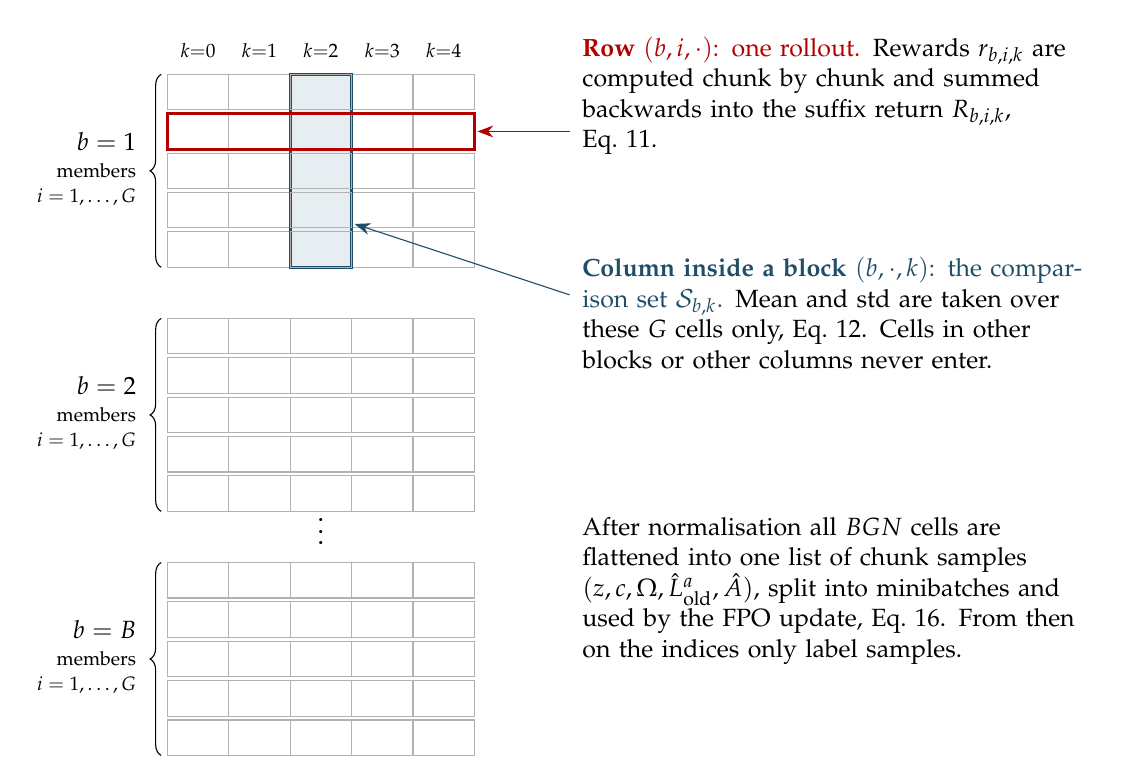
\begin{tikzpicture}[x=0.78cm,y=0.5cm,>={Stealth[length=2mm]}]
  \foreach \b/\yo/\lab in {0/0/{b=1},1/-6.2/{b=2},2/-12.4/{b=B}}{
    \foreach \i in {0,...,4}{
      \foreach \k in {0,...,4}{
        \pgfmathsetmacro{\yy}{\yo-\i}
        \draw[gray!60,fill=white] (\k,\yy) rectangle ++(1,-0.9);
      }
    }
    \node[anchor=east,font=\small,align=right] at (-0.35,\yo-2.4) {$\lab$\\[-1pt]{\scriptsize members}\\[-2pt]{\scriptsize $i=1,\dots,G$}};
    \draw[decorate,decoration={brace,amplitude=4pt,mirror}] (-0.1,\yo) -- (-0.1,\yo-4.9);
  }
  \node at (2.5,-11.4) {$\vdots$};
  \draw[very thick,blue!70!black,fill=blue!12] (2,0) rectangle (3,-4.9);
  \foreach \i in {0,...,4}{ \draw[gray!60] (2,-\i) rectangle ++(1,-0.9); }
  \draw[very thick,red!70!black] (0,-1) rectangle (5,-1.9);
  \foreach \k in {0,...,4}{ \node[font=\scriptsize] at (\k+0.5,0.6) {$k{=}\k$}; }
  \node[align=left,font=\small,anchor=north west,text width=6.4cm] (rowlab) at (6.6,1.2)
    {\textcolor{red!70!black}{\textbf{Row} $(b,i,\cdot)$: one rollout.} Rewards $r_{b,i,k}$ are computed chunk by chunk and summed backwards into the suffix return $R_{b,i,k}$, Eq.~\eqp{11}.};
  \node[align=left,font=\small,anchor=north west,text width=6.4cm] (collab) at (6.6,-4.4)
    {\textcolor{blue!70!black}{\textbf{Column inside a block} $(b,\cdot,k)$: the comparison set $\mathcal S_{b,k}$.} Mean and std are taken over these $G$ cells only, Eq.~\eqp{12}. Cells in other blocks or other columns never enter.};
  \draw[->,red!70!black] (6.55,-1.45) -- (5.05,-1.45);
  \draw[->,blue!70!black] (6.55,-5.6) -- (3.05,-3.8);
  \node[align=left,font=\small,anchor=north west,text width=6.4cm] at (6.6,-11.0)
    {After normalisation all $BGN$ cells are flattened into one list of chunk samples $(z,c,\Omega,\hat L^{a}_{\mathrm{old}},\hat A)$, split into minibatches and used by the FPO update, Eq.~\eqp{16}. From then on the indices only label samples.};
\end{tikzpicture}%

\caption{The $B\times G\times N$ batch of one update (only 5 of the 16 members are drawn per group).}
\label{loop:fig:tensor}
\end{figure}

%=====================================================================
\section{From two rewards to one number per chunk}
%=====================================================================

\subsection{Trajectory reward \eqp{8}}
For each chunk the two videos are sampled at $H_v$ common timestamps and compared view by view at the same resolution:
\begin{equation}
r^{\mathrm{traj}}_{b,i,k}=-\frac1{H_v}\sum_{t=1}^{H_v}D\big(\VC_{b,i,k,t},\VW_{b,i,k,t}\big),\qquad
D(F,F')=\frac{\|F-F'\|_2^2}{P},
\label{loop:eq:traj}
\end{equation}
with pixels on the $[0,255]$ scale and $P$ the number of compared values (channels $\times$ views $\times$ pixels). It asks: \emph{did the actions do what the policy imagined they would do?} Note that the target $\VC_{b,i,k}$ is the member's \emph{own} plan, so two members are each scored against a different target.

\subsection{Goal reward \eqp{9}}
At the last chunk only, the final Ctrl-World frame is compared with a fixed goal image (from the demonstration):
\begin{equation}
r^{\mathrm{goal}}_{b,i}=-D\big(\VW_{b,i,N-1,\mathrm{final}},\,I^\star_{g}\big).
\end{equation}
This target is \emph{the same for all members of a group}, unlike the trajectory target.

\subsection{Combined reward \eqp{10}}
\begin{equation}
r_{b,i,k}=\lambda_{\mathrm{traj}}\,r^{\mathrm{traj}}_{b,i,k}+\lambda_{\mathrm{goal}}\,\mathbf 1\{k=N-1\}\,r^{\mathrm{goal}}_{b,i}.
\label{loop:eq:reward}
\end{equation}
All rewards are $\le0$; ``higher'' means ``smaller pixel error''. The reward is a plain number: it is computed under \texttt{no\_grad}, and no gradient ever flows from it into any network. This is the first sense of the sandbox: the policy cannot change the judge (both video models are frozen), and it cannot even differentiate through the judge; it can only change which actions it samples.

\begin{codenote}[(rewards)]
\begin{itemize}[leftmargin=*]
\item The training reward is selected by \texttt{reward.training\_source}: \texttt{continuous\_combined} (\eqref{loop:eq:reward}), \texttt{trajectory\_mse}, \texttt{terminal\_goal\_mse} (the two ablation arms of Fig.~6), or \texttt{success\_binary} (a classifier reward). In the paper runs the success classifier is \emph{diagnostic only}.
\item The plotting manifest of a Push-T run lists per-camera weights for the trajectory term: wrist $2/3$, main $1/6$, side $1/6$ (and a ``no\_wrist'' variant with $0,\tfrac12,\tfrac12$). So in practice the views are \emph{not} pooled with equal weight as ``$P$ counts all values'' suggests. Check the config of the task you reproduce.
\end{itemize}
\end{codenote}

%=====================================================================
\section{Credit along a rollout: the suffix return \eqp{11}}
%=====================================================================

\subsection{Definition and matrix form}
\begin{equation}
R_{b,i,k}=\sum_{j=k}^{N-1}\gamma^{\,j-k}\,r_{b,i,j},\qquad \gamma=0.95.
\label{loop:eq:return}
\end{equation}
For $N=5$, writing the row $(b,i)$ as vectors,
\begin{equation}
\begin{pmatrix}R_0\\R_1\\R_2\\R_3\\R_4\end{pmatrix}
=\underbrace{\begin{pmatrix}
1&\gamma&\gamma^2&\gamma^3&\gamma^4\\
0&1&\gamma&\gamma^2&\gamma^3\\
0&0&1&\gamma&\gamma^2\\
0&0&0&1&\gamma\\
0&0&0&0&1
\end{pmatrix}}_{\Gamma}
\begin{pmatrix}r_0\\r_1\\r_2\\r_3\\r_4\end{pmatrix},
\qquad R=\Gamma r .
\end{equation}
The code computes this backwards, $R_{N-1}=r_{N-1}$, $R_k=r_k+\gamma R_{k+1}$ (a \texttt{done} flag would cut the recursion; with fixed-length rollouts it never does).

\subsection{What each chunk is credited for}
Inserting \eqref{loop:eq:reward} splits the return into the two sources:
\begin{equation}
R_{b,i,k}=\lambda_{\mathrm{traj}}\underbrace{\sum_{j=k}^{N-1}\gamma^{j-k}r^{\mathrm{traj}}_{b,i,j}}_{\text{own and later consistency}}
\;+\;\lambda_{\mathrm{goal}}\,\underbrace{\gamma^{\,N-1-k}\,r^{\mathrm{goal}}_{b,i}}_{\text{final outcome}} .
\label{loop:eq:split}
\end{equation}
\begin{itemize}
\item \textbf{Only the future counts.} Chunk $k$ is not credited for anything that happened before it (``suffix''), which is right: its actions cannot change the past.
\item \textbf{Every chunk sees the goal.} The goal reward reaches chunk $k$ with weight $\gamma^{N-1-k}$: $0.815,\,0.857,\,0.903,\,0.95,\,1$ for $k=0,\dots,4$. With $\gamma=0.95$ and $N=5$ the discount barely matters; it is closer to ``sum the rest of the rollout'' than to a strong preference for immediate reward.
\item \textbf{Different chunk positions have different scales.} $R_0$ sums five terms, $R_4$ only one. In the paper's laptop ablation the combined per-rollout reward is around $-12$ (Fig.~6), so $R_0$ and $R_4$ live on clearly different ranges. This is one of the reasons for normalising per chunk position (\cref{loop:sec:sandbox}).
\item \textbf{Credit is not causal.} A chunk is credited with later rewards that may be mostly due to later chunks' actions (or Ctrl-World noise). There is no critic to separate ``my contribution'' from ``what came after''; the group comparison is the only baseline.
\end{itemize}

%=====================================================================
\section{The sandbox: group-relative normalisation \eqp{12}}
\label{loop:sec:sandbox}
%=====================================================================

\subsection{Definition}
For each group $b$ and chunk position $k$, define the comparison set $\mathcal S_{b,k}=\{(b,i,k):i=1,\dots,G\}$ and
\begin{equation}
\Ah_{b,i,k}=\frac{R_{b,i,k}-\mu_{b,k}}{s_{b,k}+\delta},\qquad
\mu_{b,k}=\frac1G\sum_{i=1}^{G}R_{b,i,k},\quad
s_{b,k}=\Big(\frac1G\sum_{i=1}^{G}(R_{b,i,k}-\mu_{b,k})^2\Big)^{1/2}.
\label{loop:eq:adv}
\end{equation}
There are $B\cdot N=40$ such sets per update, each of size $G=16$. Every quantity that enters the gradient is computed \emph{inside} one set; nothing is compared across sets. This replaces the learned value function (critic) of PPO: the baseline for a chunk is ``how the other 15 members did at the same position from the same start''.

\begin{codenote}[(advantages)]
The helper \texttt{grpo\_action\_suffix\_advantages} (\texttt{src/rlinf\_modified/algorithms/advantages.py}) uses \texttt{torch.std}, which by default is the \emph{Bessel-corrected} std (divide by $G-1$), with $\delta=10^{-6}$; the implementation notes for the production path (\texttt{cross\_rank\_grpo.py}) also find that the sum of squared advantages is $G-1$. The paper says ``population'' std (divide by $G$). The difference is a constant factor $\sqrt{G/(G-1)}\approx1.03$ on all advantages, harmless but worth knowing when you reproduce numbers. Groups are spread over several GPUs (ranks), so rewards are all-gathered before \eqref{loop:eq:adv} is evaluated.
\end{codenote}

\subsection{What the sandbox cancels}
\begin{proposition}[Offsets cancel within a set]\label{loop:prop:shift}
Let $c_{b,k}$ be any numbers. Replacing $r_{b,i,k}$ by $r_{b,i,k}+c_{b,k}$ for every member $i$ leaves every advantage $\Ah_{b,i,k'}$ unchanged, for all $k'$.
\end{proposition}
\begin{proof}
By \eqref{loop:eq:return} the shift adds $\gamma^{k-k'}c_{b,k}$ to $R_{b,i,k'}$ for $k'\le k$ (and nothing for $k'>k$). The added amount does not depend on $i$, so $\mu_{b,k'}$ moves by the same amount and both $R_{b,i,k'}-\mu_{b,k'}$ and $s_{b,k'}$ are unchanged.
\end{proof}
\textbf{Consequences.}
\begin{itemize}
\item \emph{Scene difficulty cancels.} If one start scene (group $b$) gives large pixel errors for everyone (clutter, lighting, a particular duck colour), all its members are shifted together and none of them is pushed. Without grouping, every member of an easy scene would get a positive advantage and the policy would learn ``do what I did on easy scenes''.
\item \emph{Chunk-position effects cancel.} Effects common to a position (later chunks drift more because Ctrl-World conditions on its own predictions; only the last chunk carries the goal term) are removed because $k$ is never mixed.
\item \emph{The goal image's absolute distance does not matter.} Only differences between members' final frames do.
\end{itemize}

\begin{proposition}[Fixed budget per set]\label{loop:prop:budget}
If $s_{b,k}\gg\delta$, then $\sum_{i}\Ah_{b,i,k}=0$ and $\sum_i\Ah_{b,i,k}^2=G$ (or $G-1$ with Bessel's correction), independently of the rewards.
\end{proposition}
\begin{proof}
Centring gives zero sum; dividing by the std gives unit mean square.
\end{proof}
This is the ``dilution'' you noticed, and it has two faces:
\begin{itemize}
\item \textbf{Good:} every set pushes with the same strength, so a task or a scene with large reward magnitudes does not dominate the update. Multiplying all rewards by a constant $c>0$ changes nothing (up to $\delta$), so only the \emph{ratio} $\lambda_{\mathrm{goal}}/\lambda_{\mathrm{traj}}$ matters, not their overall size.
\item \textbf{Bad:} a set whose returns differ only by noise (e.g.\ Ctrl-World sampling noise, or $16$ members that all fail in nearly the same way) is pushed exactly as hard as a set with real differences. Normalisation amplifies small differences to unit scale. $\delta$ only protects against $s=0$, not against $s$ being small and meaningless. This is the reason why your thesis's referee/weighting has to think about scale (decision D1 in the implementation plan).
\end{itemize}

\begin{proposition}[Which reward term ``wins'']\label{loop:prop:mix}
Write $R_{b,i,k}=\lambda_{\mathrm{traj}}T_{b,i,k}+\lambda_{\mathrm{goal}}\gamma^{N-1-k}Y_{b,i}$ (with $Y_{b,i}=r^{\mathrm{goal}}_{b,i}$) as in \eqref{loop:eq:split}. Then
\[
\Ah_{b,i,k}=\frac{\lambda_{\mathrm{traj}}\,(T_{b,i,k}-\bar T_{b,k})+\lambda_{\mathrm{goal}}\gamma^{N-1-k}\,(Y_{b,i}-\bar Y_{b})}{s_{b,k}+\delta},
\]
so the ranking within a set is driven by $\lambda_{\mathrm{traj}}\,\mathrm{std}_i(T)$ versus $\lambda_{\mathrm{goal}}\gamma^{N-1-k}\,\mathrm{std}_i(Y)$, i.e.\ by the \emph{spread} of each term inside the group, not by its average size.
\end{proposition}
So setting $\lambda_{\mathrm{traj}}=\lambda_{\mathrm{goal}}$ does not mean ``equal importance''. If the members' final frames differ a lot (some closed the lid, some did not) while their trajectory consistency is similar, the goal term decides the advantage, and vice versa. The worked example in \cref{loop:app:toy} is exactly such a case.

\subsection{What the sandbox does \emph{not} control}
\begin{caveat}[Only chunk 0 is a clean same-state comparison]
All members share $o_{b,0}$, but $o_{b,i,1}=\mathrm{Ext}_{\mathrm{obs}}(\VW_{b,i,0})$ already differs between members. So for $k\ge1$ the set $\mathcal S_{b,k}$ compares chunks taken \emph{from different states}, with a baseline $\mu_{b,k}$ that is the same for all of them. A member that is in a worse state at $k=2$ (because of chunk 0 or 1) gets a negative advantage at $k=2$ even if its chunk-2 action was the best available from where it was. The return-to-go already carries chunk 0's consequences, so this mainly adds noise to the later-chunk updates rather than bias in the sign; still, the cleanest signal sits at $k=0$. This is the reason the thesis proposal restricts its interventional checks to chunk~0.
\end{caveat}
\begin{itemize}
\item The sandbox removes offsets \emph{common to a group}. It does not remove errors that differ between members, for instance Ctrl-World being right about one member's contact and wrong about another's. Those flip rankings, and rankings are all the gradient sees.
\item The trajectory term uses each member's \emph{own} plan as target. A member with a modest plan that is executed faithfully can outrank a member with an ambitious plan that is executed partly. The goal term is what keeps the policy from ``planning small''.
\end{itemize}

%=====================================================================
\section{Section IV.E in detail: FPO on the action head}
%=====================================================================

\subsection{Why not a normal policy gradient}
A policy gradient needs $\nabla_\theta\log\pi_\theta(a\mid c)$. For a flow model the likelihood of a sample needs the full ODE (and a trace of the Jacobian), and for UniPC, a multi-step high-order solver, there is not even a simple per-step Gaussian to write down (which Flow-GRPO and $\pi$RL need). FPO avoids all of this: it scores the \emph{endpoint} $z$ with a conditional flow-matching (CFM) loss and treats the sampler as a black box. Only the stored endpoint matters, not how UniPC reached it.

\subsection{Noising the stored endpoint \eqp{13}}
For each stored chunk, draw $Q$ probes $\Omega_{b,i,k}=\{(\tau_q,\varepsilon_q)\}_{q=1}^Q$, $\tau_q\sim\mathcal U(0,1)$, $\varepsilon_q\sim\mathcal N(0,I)$, and form
\begin{equation}
z^{(q)}=z+(1-\tau_q)\,M\odot(\varepsilon_q-z)\qquad(\text{indices }b,i,k\text{ dropped}).
\label{loop:eq:noise}
\end{equation}
At $\tau=1$ this is the clean endpoint $z$; at $\tau=0$ the masked coordinates are pure noise. Differentiating in $\tau$ gives the target velocity
\begin{equation}
\frac{\partial z^{(q)}}{\partial\tau}=M\odot(z-\varepsilon_q)=:u^{(q)},
\label{loop:eq:target}
\end{equation}
the constant ``noise-to-data'' direction of the straight path. The mask $M$ selects \textbf{both} the future video latents and the valid action coordinates; the conditioning latents (current frame) and padding stay clean. The video part is noised too because during sampling Cosmos3 denoises video and action \emph{jointly} at the same noise level; asking the action head for a velocity while the video latents were clean would query it in a situation it never sees.

\begin{codenote}[(time convention, noise, schedule)]
\begin{itemize}[leftmargin=*]
\item The code uses $\sigma=1-\tau$: $x_\sigma=x_0+\sigma(\varepsilon-x_0)$, target $\varepsilon-x_0$ ($\sigma=1$ is noise). Same path, reversed clock; signs of the target flip accordingly.
\item $\tau$ is not necessarily uniform: \texttt{fpo.time\_distribution} and a \texttt{training\_shift} $s$ map a base time $t$ to $\sigma=st/(1+(s-1)t)$ (the usual ``shifted'' schedule of video diffusion), which concentrates probes at high noise when $s>1$.
\item Probes are not stored as tensors but as integer seeds derived from the sampling seed and the probe index; $\varepsilon_q$ is regenerated from them. Before the first optimiser step the code recomputes $\Lha_{\mathrm{old}}$ and raises an error if it does not match the stored value. This guarantees the ``same probes for old and new policy'' condition.
\end{itemize}
\end{codenote}

\subsection{The action-only CFM loss \eqp{14}}
\begin{equation}
\Lha_{\tha}(z\mid c)=\frac1Q\sum_{q=1}^{Q}\Big\|P_a\big[v_{\thv,\tha}(z^{(q)},\tau_q\mid c)-u^{(q)}\big]\Big\|_2^2,\qquad c=(o_{b,i,k},g_b).
\label{loop:eq:cfm}
\end{equation}
$P_a$ keeps only the valid action coordinates of the predicted and target velocity. Read it as: \emph{how well does the current network ``explain'' this particular action as a denoising target, in this state?} A small $\Lha$ means that from noised versions of $z^a$ the network points straight back to $z^a$, so sampling in the same condition is likely to land near $z^a$.

Two things about the gradient:
\begin{itemize}
\item The velocity at the action coordinates depends on both parameter blocks (the action head attends to the video latents through the shared network), but only $\tha$ receives gradients; $\thv$ is frozen (\texttt{fpo.freeze\_video\_path}, \texttt{fpo.train\_action\_path\_only}).
\item The loss on video coordinates is not part of the objective (the code has a diagnostic \texttt{fpo\_vision\_velocity\_mse} that is explicitly excluded from the loss).
\end{itemize}

\begin{codenote}[(score parameterisation)]
\texttt{fpo.score\_parameterization} $\in\{\texttt{velocity},\texttt{epsilon}\}$. \eqref{loop:eq:cfm} is the velocity form. The epsilon form is the error of the implied noise prediction, which for the linear path is exactly $(1-\sigma)^2=\tau^2$ times the velocity error. It therefore reweights the probes: noisy probes ($\tau$ small) count much less. This changes how fast the ratio below moves and which probes dominate it, so it is a real design choice, not a detail. The code uses ``score'' $=-\Lha$, and \texttt{log\_ratio = current\_score $-$ old\_score}.
\end{codenote}

\subsection{The surrogate ratio \eqp{15} and why it is a ratio}
\begin{equation}
\hat\rho_{b,i,k}(\tha)=\exp\!\big(\Lha_{\thao}(z_{b,i,k}\mid c_{b,i,k})-\Lha_{\tha}(z_{b,i,k}\mid c_{b,i,k})\big),
\label{loop:eq:ratio}
\end{equation}
with the same endpoint, condition and probes in both losses. The justification (from the FPO paper) is that, for a suitable weighting over $\tau$, the CFM loss is, up to an additive constant and a positive factor, the negative evidence lower bound (ELBO) of the sample: $\log p_\theta(z\mid c)\gtrsim-\kappa\,L_{\mathrm{CFM},\theta}(z\mid c)+\text{const}$. The difference of two losses at the same $z$ is then a proxy for $\log p_\theta-\log p_{\mathrm{old}}$, and the constant cancels. Properties worth keeping in mind:
\begin{itemize}
\item $\hat\rho>1$ $\Leftrightarrow$ the loss on this sample went \emph{down} $\Leftrightarrow$ the new policy ``likes'' this action more.
\item It is a surrogate, not the true likelihood ratio: the bound is not tight, the weighting in practice is chosen empirically (\texttt{score\_parameterization}, schedule shift), and with finite $Q$ it is a Monte Carlo estimate. Sharing the probes between old and new (common random numbers) is what makes the \emph{difference} low-variance even when each loss is noisy.
\item The scale of $\Lha$ sets how fast $\hat\rho$ moves per parameter change: a sum over the $32\times10=320$ action coordinates moves it much faster than a mean. This interacts with the clip range like a learning rate does.
\end{itemize}

\subsection{The clipped objective \eqp{16}}
\begin{equation}
J_{\mathrm{FPO}}(\tha)=\frac1{BGN}\sum_{b,i,k}\min\Big(\hat\rho_{b,i,k}\Ah_{b,i,k},\ \clip(\hat\rho_{b,i,k},1-\epsilon_{\mathrm{clip}},1+\epsilon_{\mathrm{clip}})\,\Ah_{b,i,k}\Big).
\label{loop:eq:fpo}
\end{equation}
This is the PPO clip with the ratio replaced. Case by case:
\begin{center}
\small
\begin{tabular}{@{}llll@{}}
\toprule
Advantage & Ratio & Term used & Gradient\\
\midrule
$\Ah>0$ (better than group) & $\hat\rho\le1+\epsilon$ & $\hat\rho\Ah$ & pushes $\Lha$ down (make action more likely)\\
$\Ah>0$ & $\hat\rho>1+\epsilon$ & $(1+\epsilon)\Ah$ & \textbf{zero}: already moved enough\\
$\Ah<0$ (worse than group) & $\hat\rho\ge1-\epsilon$ & $\hat\rho\Ah$ & pushes $\Lha$ up (make action less likely)\\
$\Ah<0$ & $\hat\rho<1-\epsilon$ & $(1-\epsilon)\Ah$ & \textbf{zero}: already moved enough\\
\bottomrule
\end{tabular}
\end{center}

\subsection{The gradient, written out}
Since $\nabla\hat\rho=\hat\rho\,\nabla\log\hat\rho=-\hat\rho\,\nabla\Lha_{\tha}$,
\begin{equation}
\nabla_{\tha}J_{\mathrm{FPO}}=-\frac1{BGN}\sum_{b,i,k}\mathbf 1\{\text{not clipped}\}\;\Ah_{b,i,k}\,\hat\rho_{b,i,k}\;\nabla_{\tha}\Lha_{\tha}(z_{b,i,k}\mid c_{b,i,k}).
\label{loop:eq:grad}
\end{equation}
At the first minibatch of an update $\tha=\thao$, so $\hat\rho=1$, nothing is clipped, and
\begin{equation}
\nabla_{\tha}J_{\mathrm{FPO}}\big|_{\tha=\thao}=-\frac1{BGN}\sum_{b,i,k}\Ah_{b,i,k}\,\nabla_{\tha}\Lha_{\tha}(z_{b,i,k}\mid c_{b,i,k}).
\label{loop:eq:grad1}
\end{equation}
\begin{intuition}{The update is signed, advantage-weighted flow matching on the policy's own samples}
Compare with supervised fine-tuning, where the step is $-\eta\,\frac1n\sum\nabla L_{\mathrm{CFM}}(\text{demo action})$. Equation~\eqref{loop:eq:grad1} is the same regression, but (i) on actions the policy generated itself, in states Ctrl-World generated, and (ii) each sample is weighted by its advantage: positive weight $=$ ``regress towards this action'', negative weight $=$ ``regress away from it''. Because $\sum_i\Ah_{b,i,k}=0$ in every set (\cref{loop:prop:budget}),
\[
\sum_{i}\Ah_{b,i,k}\nabla\Lha_{b,i,k}=\sum_i\Ah_{b,i,k}\big(\nabla\Lha_{b,i,k}-\overline{\nabla\Lha}_{b,k}\big),
\]
so any gradient direction shared by all members of a set cancels. What survives is the \emph{contrast}: ``move towards the better siblings and away from the worse ones, from this start and at this position''. That is the precise sense in which the optimisation is sandboxed per $(b,k)$, even after the samples are flattened into minibatches.
\end{intuition}

\subsection{The update loop}
Algorithm~1 of the paper, made explicit:
\begin{enumerate}
\item \textbf{Freeze a behaviour copy.} $\thao\leftarrow\tha$.
\item \textbf{Roll out} $B\cdot G=128$ trajectories of $N=5$ chunks with $\thao$ through Cosmos3 (UniPC) and Ctrl-World. For each of the $640$ chunks store $z$, $c=(o,g)$, the probe seeds $\Omega$, and $\Lha_{\thao}$ (computed once, under \texttt{no\_grad}).
\item \textbf{Score}: rewards \eqref{loop:eq:reward}, returns \eqref{loop:eq:return}, advantages \eqref{loop:eq:adv}. These are now constants.
\item \textbf{Optimise}: split the 640 chunks into minibatches. For each minibatch compute $\Lha_{\tha}$ with gradients, $\hat\rho$, the clipped loss $-J$ (averaged over the minibatch), backpropagate into $\tha$ only, and take \emph{one} optimiser step (AdamW with gradient-norm clipping, per the config fields). In the code the minibatch is assembled from micro-batches on each GPU with gradient accumulation and data parallelism.
\item Because $\tha$ changes after the first minibatch, $\hat\rho\neq1$ from the second minibatch on, and that is where clipping becomes active. With a single pass and few minibatches, clipping is a mild safeguard rather than the main brake.
\item Go to 1. A production run is about 50 updates; the laptop ablation in Fig.~6 shows 15.
\end{enumerate}

\begin{codenote}[(batch and ratio variants)]
\begin{itemize}[leftmargin=*]
\item The batch is fixed by a contract: global minibatch $=$ micro-batch per GPU $\times$ world size $\times$ accumulation steps, and the number of optimiser steps per update is (trajectories $\times$ chunks)$/$global minibatch. For example, a cup profile in the tests has 512 trajectories (2560 chunks) and a global minibatch of 1280 chunks, i.e.\ 2 optimiser steps per update. Some profiles thus use larger batches than the paper's $B\cdot G=128$.
\item \texttt{fpo.ratio\_granularity} $\in\{\texttt{per\_action},\texttt{per\_mc}\}$. \eqref{loop:eq:ratio} averages the loss over the $Q$ probes \emph{before} exponentiating (one ratio per chunk). \texttt{per\_mc} forms and clips one ratio per probe; a unit test checks that the two give different losses. The PPO clip may be asymmetric (\texttt{clip\_ratio\_low}, \texttt{clip\_ratio\_high}).
\item The loss logs \texttt{approx\_kl} and \texttt{clip\_fraction}, the two numbers to watch to know whether the step size is sensible.
\end{itemize}
\end{codenote}

\subsection{What is frozen, what learns}
\begin{center}
\small
\begin{tabularx}{\linewidth}{@{}l c Y@{}}
\toprule
Component & Status & Role in the update\\
\midrule
Cosmos3 video path $\thv$ & frozen & produces $\VC$ (reward target) and the video latents the action head attends to\\
Cosmos3 action head $\tha$ & \textbf{trained} & only parameters with gradients, via $\Lha$\\
Ctrl-World $\phi^0$ & frozen & produces $\VW$ and the next observation; never differentiated\\
Goal image $I^\star_g$ & fixed & from the demonstration\\
Success classifier & frozen & diagnostics only (model-space success)\\
\bottomrule
\end{tabularx}
\end{center}
A subtle point: $\VC$ is generated jointly with $a$ from the same latent. Changing $\tha$ changes the action latents during sampling, which the video latents attend to, so the plans $\VC$ can change after training even though $\thv$ is frozen. ``The policy cannot modify the predictive models'' is true for parameters, not for the plans it is scored against.

%=====================================================================
\section{One update with numbers}
%=====================================================================
\begin{center}
\small
\begin{tabularx}{\linewidth}{@{}l Y@{}}
\toprule
Step & Paper setting\\
\midrule
Groups, members, chunks & $B=8$, $G=16$, $N=5$ $\Rightarrow$ 128 rollouts, 640 chunk samples\\
Actions per chunk & $32\times10$ at 15\,Hz (about 2.1\,s); one rollout covers about 10.7\,s of imagined time\\
Model calls & 640 Cosmos3 samples (UniPC) $+$ 640 Ctrl-World predictions\\
Rewards & 640 trajectory terms, 128 goal terms (last chunk only)\\
Comparison sets & $B\cdot N=40$ sets of 16; advantages have zero mean and unit mean square in each\\
FPO evaluations & $640\times Q$ forward passes for $\Lha_{\mathrm{old}}$, the same again with gradients\\
Optimiser steps & $640/(\text{minibatch size})$, single pass\\
Discount & $\gamma=0.95$\\
Hardware & 32 GH200 (from the authors' slides); per task 928--1396 GPU-hours, 29--43 h wall clock\\
\bottomrule
\end{tabularx}
\end{center}

%=====================================================================
\section{Experimental setup (Section V.A and around)}
%=====================================================================

\subsection{Tasks, data, trials}
\begin{center}
\small
\begin{tabular}{@{}lrrrrl@{}}
\toprule
Task & Demos & Real trials$^\dagger$ & SFT & RL & Main difficulty\\
\midrule
Laptop closing & 40 & 50 & 22.0\% & 68.0\% & contact: rotate lid, keep base still\\
Duck placing & 200 (50/colour) & 60 & 95.0\% & 100.0\% & identity from instruction (4 colours)\\
Push-T & 150 & 90 & 23.3\% & 48.9\% & pose inference, pushing\\
Cup nesting & 100 & 30 & 33.3\% & 83.3\% & longest horizon, 4 grasp-and-place\\
\bottomrule
\end{tabular}

\smallskip
{\footnotesize $^\dagger$Not stated in the paper; inferred from Table~II, where $n$ is the number of successes: $11/0.22=34/0.68=50$, $57/0.95=60/1.0=60$, $21/0.233=44/0.489=90$, $10/0.333=25/0.833=30$.}
\end{center}

\begin{itemize}
\item \textbf{Robot:} UR5 (the code's kinematics are those of the original UR5), three cameras (main, wrist, side).
\item \textbf{Split and checkpoint:} demonstrations split 4:1 train/test per task; for every method the checkpoint with lowest validation loss \emph{during adaptation} is selected. For the RL stage the paper does not say which update is deployed.
\item \textbf{Where RL data comes from:} only the first frame of each demonstration (as reset state) and its final frame (as goal image). No real transitions, no success labels.
\item \textbf{Baselines:} SFT initialisation, Fast-WAM, VLA-JEPA, $\pi_{0.5}$, each with its official training recipe and execution horizon on the same demonstrations. The weak Fast-WAM/VLA-JEPA numbers are read by the authors as ``low-data regime is hard'', not as a verdict on those methods.
\item \textbf{Metric:} real-robot success rate per task, averaged with equal task weight (43.4\%$\to$75.1\%); plus completion time and control steps over successful trials (Table~II, so the two rows cover different trial sets).
\end{itemize}

\subsection{The model-space experiments}
These are not real-robot results; all their numbers come from Ctrl-World predictions scored by a frozen instruction-conditioned success classifier on the terminal frame.
\begin{itemize}
\item \textbf{Fig.~5 (gap during SFT):} at 0.5k, 5k, 10k, 15k SFT steps, 100 paired rollouts from 20 initialisations. Imagined video ``succeeds'' 18\%$\to$50\%, Ctrl-World's rollout of the same actions 6--13\%. This 41-point gap is the motivation for the trajectory reward.
\item \textbf{Fig.~6 (reward ablation, laptop):} trajectory-only, goal-only, combined; same initialisation, sampler, FPO and budget; 15 updates. Each reward rises under its own objective; model-space success peaks at updates 9--11 and then declines for all three. The authors suggest a mismatch between the optimised policy and Ctrl-World's training distribution. There is no stopping rule in the method.
\item \textbf{Figs.~7--8 (reward vs.\ predicted success):} combined reward separates predicted successes from failures clearly on laptop and cup, weakly on duck and Push-T. Both axes come from Ctrl-World, so this checks internal consistency, not physical correctness.
\end{itemize}

\subsection{What is not in the paper (and where to find it)}
\begin{center}
\small
\begin{tabularx}{\linewidth}{@{}l Y@{}}
\toprule
Missing in the paper & Where to look in the repository\\
\midrule
$\lambda_{\mathrm{traj}},\lambda_{\mathrm{goal}}$, per-view weights & reward section of the task YAML (\texttt{reward.video\_similarity.view\_weights})\\
$Q$, time distribution, shift, score form & \texttt{fpo.num\_mc\_samples}, \texttt{fpo.time\_distribution}, \texttt{fpo.training\_shift}, \texttt{fpo.score\_parameterization}\\
$\epsilon_{\mathrm{clip}}$ & \texttt{algorithm.clip\_ratio\_low/high}\\
Learning rate, Adam betas, weight decay, grad clip & \texttt{optimizer.*}\\
Minibatch size, optimiser steps per update & \texttt{batch.global\_minibatch\_chunks}, \texttt{batch.expected\_optimizer\_steps}\\
Number of updates, deployed checkpoint & \texttt{runtime.max\_updates} (50 in the duck profiles); deployment choice not documented\\
UniPC steps, guidance & \texttt{cosmos.sampler\_steps}, \texttt{cosmos.guidance}\\
Ctrl-World denoising steps, history & \texttt{ctrl\_world.runtime.*}\\
\bottomrule
\end{tabularx}
\end{center}
The \texttt{configs/} folder is not among the synced sources of this project, so the actual values have to be read on the lab machine.

%=====================================================================
\section{Where an intervention can enter the loop}
%=====================================================================
For your thesis (a referee that distrusts some Ctrl-World feedback), the derivation above shows four places to act, with different consequences:
\begin{enumerate}
\item \textbf{Reward level}, before \eqref{loop:eq:return}: replace or down-weight $r_{b,i,k}$. By \cref{loop:prop:shift}, replacing a reward by the group's mean at that chunk is neutral for that member's centred return, but \cref{loop:prop:budget} renormalises the set, so the other members are pushed harder (decision D1).
\item \textbf{Advantage level}, after \eqref{loop:eq:adv}: scale $\Ah_{b,i,k}$ by a trust weight $w\in[0,1]$. This changes the push size directly and does not touch other members; it breaks the zero-sum property of the set.
\item \textbf{Mask level}, inside \eqref{loop:eq:fpo}: drop a sample from the average (the code's \texttt{loss\_mask}). Equivalent to $w=0$ at advantage level.
\item \textbf{Set level}: skip whole sets $\mathcal S_{b,k}$ whose spread $s_{b,k}$ is not larger than the noise level (e.g.\ estimated from repeated Ctrl-World calls with different seeds), which addresses the amplification of meaningless differences.
\end{enumerate}

%=====================================================================
\section{A worked example}
\label{loop:app:toy}
%=====================================================================
One group, $G=4$ members, $N=3$ chunks, $\gamma=0.95$, $\lambda_{\mathrm{traj}}=\lambda_{\mathrm{goal}}=1$. Trajectory rewards per chunk and goal rewards:
\begin{center}
\small
\begin{tabular}{@{}c rrr r@{}}
\toprule
$i$ & $r^{\mathrm{traj}}_{i,0}$ & $r^{\mathrm{traj}}_{i,1}$ & $r^{\mathrm{traj}}_{i,2}$ & $r^{\mathrm{goal}}_i$\\
\midrule
1 & $-4.0$ & $-4.2$ & $-4.5$ & $-6.0$\\
2 & $-4.4$ & $-4.6$ & $-5.0$ & $-7.5$\\
3 & $-3.9$ & $-4.0$ & $-4.1$ & $-5.5$\\
4 & $-4.3$ & $-4.8$ & $-5.2$ & $-7.0$\\
\bottomrule
\end{tabular}
\end{center}
Combined rewards: $r_{i,2}=r^{\mathrm{traj}}_{i,2}+r^{\mathrm{goal}}_i$, e.g.\ $r_{1,2}=-10.5$. Returns (backwards) and advantages (population std, as in the paper):
\begin{center}
\small
\begin{tabular}{@{}c rrr rrr@{}}
\toprule
& \multicolumn{3}{c}{$R_{i,k}$} & \multicolumn{3}{c}{$\Ah_{i,k}$}\\
\cmidrule(lr){2-4}\cmidrule(lr){5-7}
$i$ & $k=0$ & $k=1$ & $k=2$ & $k=0$ & $k=1$ & $k=2$\\
\midrule
1 & $-17.47$ & $-14.18$ & $-10.50$ & $+0.62$ & $+0.60$ & $+0.58$\\
2 & $-20.05$ & $-16.48$ & $-12.50$ & $-1.03$ & $-1.00$ & $-1.09$\\
3 & $-16.36$ & $-13.12$ & $-9.60$ & $+1.32$ & $+1.33$ & $+1.34$\\
4 & $-19.87$ & $-16.39$ & $-12.20$ & $-0.91$ & $-0.94$ & $-0.84$\\
\midrule
$\mu_k$ & $-18.44$ & $-15.04$ & $-11.20$ & \multicolumn{3}{c}{$\sum_i\Ah=0$, $\sum_i\Ah^2=4$ per column}\\
$s_k$ & $1.57$ & $1.44$ & $1.20$ & & &\\
\bottomrule
\end{tabular}
\end{center}
Observations:
\begin{itemize}
\item The means differ by almost 7 between $k=0$ and $k=2$ only because $R_0$ sums more terms; normalising per position removes this.
\item The goal rewards spread by about $0.8$ (std), the per-chunk trajectory rewards by about $0.2$--$0.4$. The ranking ($3>1>4>2$) is essentially the goal ranking: \cref{loop:prop:mix} in action, although $\lambda_{\mathrm{traj}}=\lambda_{\mathrm{goal}}$.
\item With Bessel's correction (the code), every advantage is multiplied by $\sqrt{3/4}\approx0.87$ for $G=4$ (by $\approx0.97$ for $G=16$); the signs and the ranking do not change.
\item If all four members had rewards within $\pm0.01$ of each other (pure noise), the advantages would still have unit mean square: the same push, on noise.
\end{itemize}


% Chapter 02. Source: docs/book/import/fpo_from_zero.tex, ported in D.2 without rewriting. Its
% four images are regenerated by scripts/make_book_figures.py into docs/book/figures/.
% Skeleton from WP D.1: the section headings below are the source's; D.2 replaces them with its body.
\chapter{From policy gradients to FPO}\label{ch:rl-to-fpo}

\section*{The road map in one paragraph}

\section{Mathematical toolkit beyond Calculus I--II}

\section{The reinforcement-learning problem}

\section{Two families of methods, and why the paper uses policy search}

\section{Policy-gradient methods}

\section{PPO: improving the policy in safe steps}

\section{GRPO: advantages without a critic}

\section{Flow models from zero, and why PPO cannot be used directly}

\section{FPO: the CFM loss as a stand-in for the log-probability}

\section{Mapping onto the paper's Eqs.~(13)--(16)}

\section*{Glossary}

% Chapter 03. Source: import/thesis_proposal_final.tex (final version, 27 Oct 2026), Sections 1-14
% with the box "The proposal in brief", taken as they are (D.2): the wording is not changed. Removed:
% the title block (title = the book's title; subtitle and date are the \sourcenote) and the table
% of contents. Labels prefixed with method:, the two TikZ pictures in figures/03_*.tex. The
% proposal's appendix (Notation) is the book's Appendix A (chapters/A_notation.tex), its
% references are docs/book/bibliography.tex. Numbering: the code's docstrings cite the proposal's
% Section, Step, equation and proposition numbers, so this chapter prints the same ones (sections
% without the chapter prefix; equations and theorems are counted per chapter, see preamble.tex).
\chapter{The thesis proposal}\label{ch:proposal}
\sourcenote{A physics-twin referee for robot policies trained inside a learned world model.\\
Master thesis proposal, final version, 27 October 2026.}
\renewcommand{\thesection}{\arabic{section}}
\begin{keybox}[title={\textbf{The proposal in brief}},fonttitle=\color{white}\bfseries,colbacktitle=blue!60!black]
\textbf{Context.} \emph{Achieve What You Imagined}~\cite{a2a} trains the action head of a world-action model (Cosmos~3~\cite{cosmos3}) with reinforcement learning (FPO~\cite{fpo}) entirely in imagination: the reward compares the policy's imagined plan with what a frozen action-conditioned world model (Ctrl-World~\cite{ctrlworld}) predicts its actions will do. Real success on four UR5 tasks rises from 43.4\% to 75.1\% without any robot interaction during training.

\textbf{Problem.} The reward is only as good as Ctrl-World's predictions. Where those predictions are physically wrong, mostly at contact, the policy is optimised against the model's errors, and nothing in the loop can detect it. The paper's own success in imagination peaks after 9--11 updates and then declines, without an identified cause.

\textbf{Research question.} \emph{Can checking a world model's feedback against a physics twin of the scene make robot policies trained in imagination more reliable in the real world?} Split into RQ1 \emph{Detect}, RQ2 \emph{Explain}, RQ3 \emph{Improve} (Section~\ref{method:sec:rq}).

\textbf{Method.} A simple MuJoCo twin of the scene is initialised automatically from the real first camera frame (SAM~3 segmentation and a render-and-compare fit) and receives exactly the same actions as Ctrl-World. At the first chunk, controlled action interventions give a per-reward verdict (consistent, wrong reaction, ignores the action, invents an effect, or no verdict). At later chunks, the twin runs open-loop from the real start alongside Ctrl-World, and a calibrated test detects when Ctrl-World's scene has left what physics allows. Each reward is then weighted by this trust, in a way that provably reduces to the paper when trust is full and removes a distrusted reward's influence exactly when trust is zero.

\textbf{Deliverables and real-world demonstrations.} (G1) the referee as open code, validated on real first frames of all four tasks and on replays of the 40 laptop demonstrations; (G2) an audit of where and when the world model is wrong, plus about 20 real action pairs on the UR5 showing which model predicts reality; (G3) a trust-weighted laptop-closing policy compared with the paper's policy on the UR5, about 60 trials each.
\end{keybox}

%=====================================================================
\section{Introduction}
%=====================================================================
Real robot data is expensive: the paper's tasks have 40--200 demonstrations each, and every real reinforcement-learning trial costs minutes of robot time and a person to reset the scene. Learned video world models offer an alternative: a policy can try thousands of rollouts inside the model and be improved without touching the robot. \emph{Achieve What You Imagined}~\cite{a2a} shows that this works on a real UR5.

A policy optimised against a model is also optimised against the model's errors. This is well known in model-based reinforcement learning~\cite{mopo,exploitable}: wherever the model is too optimistic, the optimiser will find it. Learned video models are least reliable exactly where manipulation happens, at contact: the Ctrl-World authors report imprecise modelling of collisions, sliding and rotations, including on laptop closing~\cite{ctrlworld}. Nothing in the paper's training loop checks whether the world model's predicted consequence is physically possible.

This thesis adds such a check. The world model is cross-checked against an \emph{independent} model of the same scene, a physics simulation, which has the opposite error profile: visually crude, but physically consistent by construction. The two are run on the same actions from the same real start. Where the simulator's answer does not depend on what it does not know, disagreement is evidence that the world model's feedback is wrong, and that feedback is down-weighted in training.

\paragraph{Related work.} World-model-based policy optimisation for vision-language-action models (e.g.\ WMPO~\cite{wmpo}) and the base paper~\cite{a2a} train against learned video models without an external physical check. Penalising model uncertainty is the classical remedy in model-based offline RL~\cite{mopo}, and recent work shows that imperfect world models are systematically exploited by the policies trained in them~\cite{exploitable}. Digital twins have been used to evaluate real-world policies~\cite{realissim} and to ground video prediction for planning~\cite{vptwin}. This thesis uses a twin for a different purpose: as an independent \emph{referee} of a learned world model's feedback during training, with verdicts that abstain when the twin's own uncertainty matters and a false-alarm rate calibrated on real demonstrations.

The thesis measures before it intervenes. RQ1 and RQ2 are measurements: how often and where the world model contradicts physics, and whether those errors grow during training and explain the decline. They are results whatever happens to RQ3, the method. All three are tied to concrete measurements on real data or on the real robot.

\paragraph{Structure.} Section~\ref{method:sec:background} describes the paper's loop and two facts about it on which the method rests. Section~\ref{method:sec:problem} states the problem. Section~\ref{method:sec:rq} gives the research goal, the research question, its three sub-questions and the hypotheses. Section~\ref{method:sec:scope} fixes the setting and scope. Section~\ref{method:sec:method} describes the method step by step, with well-posedness arguments where a quantity could be ill defined. Section~\ref{method:sec:assumptions} lists the assumptions and how each is tested. Sections~\ref{method:sec:experiments}--\ref{method:sec:expected} describe experiments, deliverables, real-world demonstrations and expected results. Sections~\ref{method:sec:risks}--\ref{method:sec:decisions} cover risks, budget, work plan and open decisions. Notation is collected in Appendix~\ref{method:app:notation}.

%=====================================================================
\section{Background: the training loop this thesis builds on}\label{method:sec:background}
%=====================================================================

\subsection{Models and data}
\begin{itemize}
\item \textbf{World-action model (policy).} Cosmos3-Nano fine-tuned on UR5 demonstrations~\cite{cosmos3,a2a}. It generates a video plan and an action chunk jointly. Its video path is frozen; only the action head, parameters $\theta_a$, is trained.
\item \textbf{World model.} Ctrl-World~\cite{ctrlworld}, an action-conditioned video diffusion model fine-tuned on the task's UR5 data, frozen during RL. It takes the current multi-view observation, a short history and an action chunk, and predicts the multi-view video those actions would produce.
\item \textbf{Data.} For laptop closing, 40 demonstrations (32 used as training starts) with three camera views (wrist, front, side), robot states and actions.
\item \textbf{Real inputs to RL.} Only the first frame of each training demonstration (start) and its final frames (goal image). No robot interaction.
\end{itemize}

\subsection{One RL iteration, step by step}
A rollout has $N=5$ chunks $k=0,\dots,N-1$. Rollouts come in groups of $G=16$ candidates $i=1,\dots,G$ that share the start observation $o_0$ and instruction $g$ (``close the laptop'').

\textbf{Step B1: imagine and act.} At chunk $k$ the policy samples a latent and decodes a plan video and an action chunk,
\begin{equation}
z_{i,k}\sim\Pi_\theta(\cdot\mid o_{i,k},g),\qquad (\VC_{i,k},\,a_{i,k})=D(z_{i,k}),
\end{equation}
with $a_{i,k}\in\R^{H_a\times d_a}$, $H_a=32$ steps at 15\,Hz, and $d_a=10$ (relative end-effector translation and rotation, gripper).

\textbf{Step B2: predict the consequence.} Ctrl-World receives the same actions, converted to its input format by $T_a$, and predicts the video; its last frame becomes the next observation:
\begin{equation}
(\VW_{i,k},h_{i,k+1})=W\big(h_{i,k},T_a(a_{i,k}),\xi\big),\qquad o_{i,k+1}=\mathrm{Ext}(\VW_{i,k}),
\end{equation}
where $h$ is Ctrl-World's conditioning state (current and history frames with robot poses) and $\xi$ its sampling noise. From chunk~1 on, the policy sees only generated images.

\textbf{Step B3: reward.} The reward compares imagined and predicted frames, plus a goal term at the last chunk:
\begin{equation}\label{method:eq:reward}
r_{i,k}=-\frac{\lambda_{\mathrm{traj}}}{H_v}\sum_{t=1}^{H_v}D_{\mathrm{pix}}\big(\VC_{i,k,t},\VW_{i,k,t}\big)\;-\;\lambda_{\mathrm{goal}}\,\mathbf 1\{k=N-1\}\,D_{\mathrm{pix}}\big(\VW_{i,N-1,\mathrm{final}},I^\star_g\big),
\end{equation}
with $D_{\mathrm{pix}}$ the pixel mean squared error, $I^\star_g$ the goal image and $\lambda_{\mathrm{traj}},\lambda_{\mathrm{goal}}\ge 0$.

\textbf{Step B4: returns and advantages.} With discount $\gamma=0.95$,
\begin{equation}\label{method:eq:adv}
R_{i,k}=\sum_{j=k}^{N-1}\gamma^{\,j-k}r_{i,j},\qquad
\hat A_{i,k}=\frac{R_{i,k}-\mu_k}{s_k+\epsilon_{\mathrm{num}}},\qquad
\mu_k=\tfrac1G\textstyle\sum_iR_{i,k},\quad s_k=\Std_i R_{i,k}.
\end{equation}

\textbf{Step B5: update.} FPO~\cite{fpo} maximises the clipped surrogate $\E\big[\min(\rho\hat A,\,\mathrm{clip}(\rho,1\pm\epsilon_{\mathrm{clip}})\hat A)\big]$, where $\rho=\exp(\hat L_{\mathrm{old}}-\hat L_\theta)$ is built from conditional flow-matching losses of the action head. A production run has about 50 updates.

\subsection{Two facts the method rests on}
\begin{lemma}[Only within-group differences matter]\label{method:lem:shift}
Adding the same constant $c_k$ to the reward of every candidate at chunk $k$ leaves all advantages $\hat A_{i,k'}$ unchanged.
\end{lemma}
\begin{proof}
The shift adds $\gamma^{k-k'}c_k$ to every $R_{i,k'}$ with $k'\le k$, the same for all $i$, so $\mu_{k'}$ shifts by the same amount and both $R_{i,k'}-\mu_{k'}$ and $s_{k'}$ are unchanged. For $k'>k$ nothing changes.
\end{proof}
\begin{lemma}[Zero advantage, zero push]\label{method:lem:zero}
At the start of an update ($\theta=\theta_{\mathrm{old}}$, $\rho=1$), a sample with $\hat A_{i,k}=0$ contributes zero gradient.
\end{lemma}
\begin{proof}
At $\rho=1$ the clip is inactive and the term is $\rho\hat A$, with gradient $\hat A\,\nabla_\theta\rho=0$.
\end{proof}
\begin{why}
\textbf{Consequences.} By Lemma~\ref{method:lem:shift}, the policy learns only from \emph{which candidate is better than which}, so the right thing to check is a \emph{difference} between candidates or actions, not an absolute reward. By Lemma~\ref{method:lem:zero}, a reward set equal to the group mean stops pushing the policy; trust weighting (\ref{method:sec:trust}) uses exactly this.
\end{why}

%=====================================================================
\section{Problem statement}\label{method:sec:problem}
%=====================================================================

\subsection{The reward cannot tell whose fault a gap is}
A gap between the plan $\VC$ and the prediction $\VW$ has three possible causes:
\begin{enumerate}[label=(\alph*)]
\item \textbf{the action misses the plan}: the policy's fault, what the reward should punish;
\item \textbf{Ctrl-World mispredicts}: the world model's fault, and the reward is wrong;
\item \textbf{the plan is unrealistic}: Cosmos imagined something no action achieves.
\end{enumerate}
The reward is a single number and cannot separate them. Case (b) is the one that trains the policy toward the model's errors.

\subsection{The error is bounded by something the loop never measures}
Let $V^\ast_{i,k}$ be what the actions really do, and let $D$ be a metric (e.g.\ root mean squared pixel error). With $r^{\ast}$ the reward computed with $V^\ast$ in place of $\VW$, the reverse triangle inequality gives, for the trajectory term,
\begin{equation}\label{method:eq:bound}
\big|\,r^{\mathrm{traj}}_{i,k}-r^{\mathrm{traj},\ast}_{i,k}\big|\;\le\;\frac{1}{H_v}\sum_{t}D\big(\VW_{i,k,t},V^\ast_{i,k,t}\big).
\end{equation}
The right-hand side, the world model's prediction error, is never measured during training. By Lemma~\ref{method:lem:shift}, what actually harms learning is error that differs between candidates and so changes their ranking.

\subsection{Exploitation and the observed decline}
Policy optimisation concentrates the policy where the reward is high. Where the reward is high because of a prediction error, the policy moves toward actions whose predicted consequences are flattering but wrong. The paper's model-space success peaks after 9--11 updates and then declines for every reward variant (its Fig.~6). Whether this is exploitation of Ctrl-World, degradation of the plans, or something else is not known, because nothing in the loop measures (b).

%=====================================================================
\section{Research goal, research question and hypotheses}\label{method:sec:rq}
%=====================================================================

\begin{rqbox}[title={Research goal}]
Detect physically inconsistent world-model feedback and keep it out of policy training, using an independent physics simulation of the scene that is initialised from the real camera frame and run on the same actions.
\end{rqbox}

\begin{rqbox}[title={Research question}]
Can checking a world model's feedback against a physics twin of the scene make robot policies trained in imagination more reliable in the real world?
\end{rqbox}

The question is answered in three steps. Each step has its own kind of answer.

\begin{description}[leftmargin=0pt,itemsep=3pt]
\item[RQ1 · Detect.] \emph{How often, and where, do the world model's predicted consequences contradict physics?} Which kind of error (it reacts the wrong way to an action, ignores the action, or invents an effect that has no cause), and in which phase of the task (before, during or after contact).
\item[RQ2 · Explain.] \emph{Do these errors grow as the policy trains, and do they explain why imagined success later declines?} In particular: does the policy learn to exploit the world model, i.e.\ do rollouts that the world model and its success classifier judge successful increasingly turn out to be physically inconsistent?
\item[RQ3 · Improve.] \emph{If the policy learns only from feedback the twin trusts, does it succeed more often on the real robot?} Compared with the paper's method, on the real UR5.
\end{description}

\paragraph{Hypotheses.} The thresholds below are fixed before any RL run.
\begin{hypothesis}[Detect]\label{method:h:detect}
On rollouts of the original method, a non-trivial share (at least 10\%) of chunk-0 rewards that receive a twin verdict are failures, concentrated during gripper--lid contact.
\end{hypothesis}
\begin{hypothesis}[Referee validity]\label{method:h:valid}
On replays of held-out real demonstrations, the twin's predicted change is closer to the real change than Ctrl-World's during and after contact; on about 20 real action pairs, the twin's decisive verdicts agree in sign with the real effect more often than Ctrl-World's.
\end{hypothesis}
\begin{hypothesis}[Explain]\label{method:h:explain}
Under the original method, the rate of failures and of flagged divergences increases over updates, and its increase precedes the decline in model-space success; the share of imagined successes that are physically inconsistent increases.
\end{hypothesis}
\begin{hypothesis}[Improve]\label{method:h:improve}
At equal training budget, trust-weighted training removes or delays the late decline, and the resulting policy's real success on laptop closing is at least the paper's 68\%, with a clear improvement as target; a control with the same weights assigned at random does not improve.
\end{hypothesis}

\paragraph{What counts as an answer.} If RQ1 finds the world model rarely contradicts physics on this task, that is a finding: the decline then has another cause (e.g.\ cause (c)), and RQ3 is expected to show no gain. If RQ1 finds errors that do not grow, the world model is wrong but not exploited, and trust weighting acts as noise reduction. If errors grow and precede the decline (H\ref{method:h:explain}), the decline is explained by exploitation, and RQ3 tests whether removing that feedback fixes it.

%=====================================================================
\section{Setting and scope}\label{method:sec:scope}
%=====================================================================

\paragraph{Same models as the paper.} The authors' UR5 Cosmos3-Nano policy, the task-specific frozen Ctrl-World and the success-monitoring classifier, as released. Only the action head is trained; nothing in the video path or in Ctrl-World is changed. Results are directly comparable with the paper.

\paragraph{Main task: laptop closing.} A hinged lid is largely kinematic, so a simple simulator models it reliably; pushing tasks depend strongly on friction, which would make the referee itself unreliable. Laptop closing also has the largest RL gain in the paper (22\%$\,\to\,$68\%) and a known difficulty for Ctrl-World. The initialiser (\ref{method:sec:init}) is additionally validated on the first frames of all four tasks of the paper, to show the method is not task-specific.

\paragraph{Physics engine: MuJoCo.} MuJoCo~\cite{mujoco} runs on CPUs next to the training job on the cluster; a UR5e model is available in MuJoCo Menagerie~\cite{menagerie}. Isaac Sim was considered (it was suggested by the paper's authors), but it requires GPUs with RT cores, which the cluster's GH200 nodes lack. For the comparisons used here the physics engine only needs rigid bodies, a hinge and contacts.

\paragraph{No state is read from generated frames in the training signal.} The twin is initialised from the \emph{real} first frame only, and from then on receives only actions. Generated frames are compared with twin renders through generic video features, never parsed into object states. This keeps the training signal free of task-specific perception of generated images, and keeps the twin independent of the world model's mistakes.

\paragraph{Boundary with a colleague's thesis.} This thesis does not embed physical information into the world-action model, and introduces no goal representation, hindsight relabelling, curriculum or real-robot training data. The twin is used only to \emph{check} the existing feedback.

\paragraph{Constraints.} Hand-in 19 February 2027. Robot access from 25 January 2027 (worst case 1 February). The student works about 1400\,km from the lab: real-robot sessions are executed by lab members following a written protocol and scripts provided by the student. Compute: two RTX\,4090, one RTX\,5090, and the NAISS Arrhenius cluster (about 24k GPU-hours per month, queued).

%=====================================================================
\section{Method, step by step}\label{method:sec:method}
%=====================================================================
\renewcommand{\thesubsection}{Step~\arabic{subsection}}
\renewcommand{\thesubsubsection}{\arabic{subsection}.\arabic{subsubsection}}

\subsection*{Overview}
\addcontentsline{toc}{subsection}{Overview}
Figure~\ref{method:fig:pipeline} shows the loop. The paper's path (policy $\to$ Ctrl-World $\to$ reward $\to$ next observation) is unchanged. A second path takes the \emph{same} actions to a physics twin started from the \emph{same} real frame. The two predictions are compared through how the scene changes over time; the comparison produces a trust weight for each reward.

\begin{figure}[h]
\centering
% The figure "method:fig:pipeline" of import/thesis_proposal_final.tex, moved here unchanged in D.2;
% \input by chapters/03_method.tex. The final % keeps the spacing of the original.
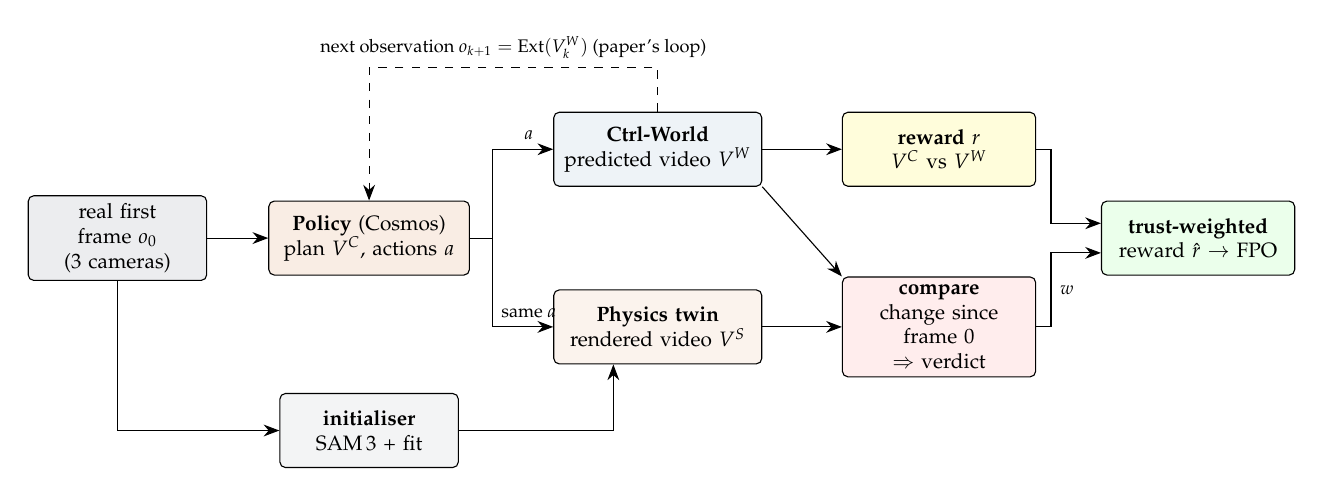
\begin{tikzpicture}[scale=0.94,transform shape,
  box/.style={draw,rounded corners=2pt,align=center,font=\footnotesize,minimum height=10mm,inner sep=3pt,text width=#1},
  box/.default=24mm,
  >={Stealth[length=2mm]}]
\node[box=22mm,fill=navy!8] (o0) at (0,0) {real first frame $o_0$\\ (3 cameras)};
\node[box=25mm,fill=orange!12] (pol) at (3.4,0) {\textbf{Policy} (Cosmos)\\ plan $\VC$, actions $a$};
\node[box=26mm,fill=blue!8] (wm) at (7.3,1.2) {\textbf{Ctrl-World}\\ predicted video $\VW$};
\node[box=26mm,fill=orange!8] (tw) at (7.3,-1.2) {\textbf{Physics twin}\\ rendered video $\VS$};
\node[box=24mm,fill=yellow!14] (rew) at (11.1,1.2) {\textbf{reward} $r$\\ $\VC$ vs $\VW$};
\node[box=24mm,fill=red!7] (cmp) at (11.1,-1.2) {\textbf{compare}\\ change since frame 0\\ $\Rightarrow$ verdict};
\node[box=24mm,fill=green!8] (tr) at (14.6,0) {\textbf{trust-weighted}\\ reward $\hat r$ $\to$ FPO};
\node[box=22mm,fill=navy!5] (ini) at (3.4,-2.6) {\textbf{initialiser}\\ SAM\,3 + fit};
\draw[->] (o0) -- (pol);
\draw[->] (pol.east) -- ++(3mm,0) |- (wm.west) node[pos=0.8,above,font=\scriptsize]{$a$};
\draw[->] (pol.east) -- ++(3mm,0) |- (tw.west) node[pos=0.8,above,font=\scriptsize]{same $a$};
\draw[->] (o0.south) |- (ini.west);
\draw[->] (ini.east) -| ([xshift=-6mm]tw.south);
\draw[->] (wm) -- (rew);
\draw[->] (wm.south east) -- (cmp.north west);
\draw[->] (tw) -- (cmp);
\draw[->] (rew.east) -- ++(2mm,0) |- ([yshift=2mm]tr.west);
\draw[->] (cmp.east) -- ++(2mm,0) |- ([yshift=-2mm]tr.west) node[pos=0.25,right,font=\scriptsize]{$w$};
\draw[->,dashed] (wm.north) -- ++(0,6mm) -| node[pos=0.25,above,font=\scriptsize]{next observation $o_{k+1}=\mathrm{Ext}(\VW_k)$ (paper's loop)} (pol.north);
\end{tikzpicture}%

\caption{The paper's loop (top, unchanged) and the added referee path (bottom). The twin starts once from the real first frame through the initialiser and from then on receives only the actions; it never sees generated frames.}
\label{method:fig:pipeline}
\end{figure}

The method has nine steps. Steps~1--3 build the referee (once per task, plus once per starting scene). Step~4 defines the comparison. Step~5 calibrates everything on real demonstrations \emph{before} any RL. Steps~6--8 run inside each RL iteration. Step~9 adds diagnostics used only for analysis.

%---------------------------------------------------------------------
\subsection{The general twin (built once per task)}\label{method:sec:twin}
The general twin is everything that is the same for every starting scene of a task:
\begin{equation}
\mathcal T=\big(\text{robot model},\ \text{table},\ \text{object model with configuration space }\X,\ \{K_v,T_v\}_{v=1}^{3},\ p(\psi)\big).
\end{equation}
\begin{itemize}
\item \textbf{Robot:} the UR5e from MuJoCo Menagerie~\cite{menagerie} with the lab's gripper (link parameters adapted if the lab robot is the older UR5).
\item \textbf{Object:} for laptop closing, the laptop as two boxes (base and lid) joined by a hinge. Its configuration is $x=(p_x,p_y,\varphi,\vartheta)\in\X$: base position on the table, base yaw, lid angle. $\X$ is the table region $\times$ yaw circle $\times$ $[\vartheta_{\min},\vartheta_{\max}]$, a compact set.
\item \textbf{Cameras:} intrinsics $K_v$ and extrinsics $T_v$ of the three cameras. If calibration files are not in the dataset, the extrinsics are estimated from the demonstrations by fitting the rendered robot (at its recorded joint angles) to the robot's segmentation masks, which needs no lab visit.
\item \textbf{Uncertain physics $\psi$:} hinge friction and damping, gripper--lid and laptop--table friction. They are not fixed but described by a belief $p(\psi)$ fitted on demonstrations (Step~5); $\Psi_K$ denotes $K$ samples from it.
\end{itemize}
The twin is deliberately simple. It is not meant to look real or to be accurate everywhere; it is meant to be \emph{physically consistent} and to know what it does not know.

%---------------------------------------------------------------------
\subsection{Initialising the twin from the first frame}\label{method:sec:init}
The twin must start in the same scene as the real first frame. The robot's joint angles $q_0$ are recorded and the scene is at rest, so only the object configuration $x_0$ is unknown. The procedure is general; only Step~2.0 changes between tasks.

\begin{center}\small
\begin{tabularx}{\linewidth}{@{}>{\raggedright\arraybackslash}p{2.6cm}>{\raggedright\arraybackslash}X>{\raggedright\arraybackslash}p{4.6cm}@{}}
\toprule
\textbf{Step} & \textbf{General procedure (any task)} & \textbf{Laptop closing (this project)}\\
\midrule
2.0 Task config (once per task) & Text prompts naming the objects and parts; a MuJoCo model of each object (primitives, or a mesh reconstructed with SAM\,3D~\cite{sam3d}); the unknown state variables and their ranges. & ``laptop'', ``laptop screen''; two boxes and a hinge; $x=(p_x,p_y,\varphi,\vartheta)$.\\
2.1 Segment & SAM\,3~\cite{sam3}, an open-vocabulary segmentation model, is run with the text prompts on each camera image of the real first frame, giving one mask per object part. Robot pixels are removed by rendering the robot at the known $q_0$. & Masks of base and screen in the three views.\\
2.2 Fit & The twin's object is rendered from each calibrated camera; the unknowns are adjusted until the rendered masks overlap the SAM\,3 masks in all views (eq.~\ref{method:eq:fit}). & Four numbers; robot pose known.\\
2.3 Physical check & The fitted scene is simulated briefly with the robot still; fits that interpenetrate or move are rejected or moved to the nearest resting configuration. & Base flat on the table, lid at rest.\\
2.4 Ambiguity & All fits nearly as good as the best are kept; every later verdict must hold for all of them, otherwise the twin gives none. & E.g.\ lid angle poorly determined when the screen is seen edge-on.\\
\bottomrule
\end{tabularx}
\end{center}

\textbf{The fit.} With $M^{\mathrm{obs}}_v$ the observed masks, $M_v(x;q_0)$ the rendered ones, $P$ observed 3D points of the object if depth or triangulation is available, $\mathcal S(x)$ the object's surface and $\mathrm{pen}(x)\ge0$ its penetration into the table:
\begin{equation}\label{method:eq:fit}
\mathcal L(x)=\sum_{v=1}^{3}\Big[1-\IoU\big(M_v(x;q_0),M^{\mathrm{obs}}_v\big)\Big]+\lambda_d\,\frac{1}{|P|}\sum_{p\in P}\min\big(\mathrm{dist}(p,\mathcal S(x)),d_{\max}\big)+\lambda_c\,\mathrm{pen}(x).
\end{equation}
The depth term is optional ($\lambda_d=0$ without depth). The estimate and the near-optimal set are
\begin{equation}
\hat x=\argmin_{x\in\X_h}\mathcal L(x),\qquad \hat\X_\nu=\{x\in\X_h:\ \mathcal L(x)\le\mathcal L(\hat x)+\nu\},
\end{equation}
where $\X_h\subset\X$ is a search grid refined around the best points and $\nu$ a tolerance. If $\mathcal L(\hat x)>\mathcal L_{\max}$, the frame is flagged and excluded.

\begin{proposition}[The fit is well posed]\label{method:prop:fit}
(a) A minimiser $\hat x$ exists and $\hat\X_\nu$ is non-empty. (b) If the grid is replaced by $\X$ and IoU by a soft IoU on blurred silhouettes, $\mathcal L$ is continuous on the compact set $\X$ and a minimiser still exists.
\end{proposition}
\begin{proof}
(a) $\X_h$ is finite and every term of $\mathcal L$ is bounded (IoU in $[0,1]$, distances capped at $d_{\max}$, penetration bounded on a bounded region), so a minimum over a finite set exists and belongs to $\hat\X_\nu$. (b) $\X$ is a product of a closed bounded region, a circle and a closed interval, hence compact; soft rasterisation of a rigid template is continuous in $x$, and so are the capped distance and the penetration depth. Weierstrass' theorem gives a minimiser.
\end{proof}
\begin{remark}[Uniqueness is not needed]
The minimiser need not be unique (the base is nearly symmetric; a single view confuses lid angle and distance). The method never relies on $\hat x$ alone: verdicts must hold for every start state in $\hat\X_\nu$, so an ambiguous frame leads to abstention rather than a wrong verdict.
\end{remark}

\textbf{Validation of the initialiser (part of G1).} (i) Leave-one-view-out: fit on two cameras, render in the third, measure IoU with that camera's mask. (ii) About 10 manually labelled frames per task give errors in degrees and centimetres. (iii) Generality: the same code, with only Step~2.0 changed, is run on real first frames of the paper's four tasks (laptop, duck, Push-T, cups).

%---------------------------------------------------------------------
\subsection{Running the same actions in the twin}\label{method:sec:dyn}
The twin's robot executes the same action chunks. They are converted by $T_S$ into joint targets (inverse kinematics of the relative end-effector motion) and tracked by a controller model whose delay and gains are fitted on the demonstrations (commanded versus measured poses). For each element $\vartheta=(\psi,x_0)$ of the uncertainty set
\begin{equation}
\Theta=\Psi_K\times\hat\X_\nu,
\end{equation}
the twin state evolves deterministically:
\begin{equation}
s_{i,0}(\vartheta)=(q_0,0,x_0,0),\qquad s_{i,k+1}(\vartheta)=F_\psi\big(s_{i,k}(\vartheta),T_S(a_{i,k})\big),\qquad \VS_{i,k}(\vartheta)=\big(\mathrm{Rend}_v(s_{i,k,t}(\vartheta))\big)_{v,t}.
\end{equation}
The twin has no sampling noise; all its uncertainty is in $\vartheta$. Parameter samples under which the observed start would not be at rest (e.g.\ hinge friction too low to hold the lid at its observed angle) contradict the real frame and are discarded for that scene.

\textbf{Rendering.} To reduce the visual gap, the real first frame is projected onto the twin's objects as texture: at $t=0$ the render nearly reproduces the real image, and later frames show these surfaces moving. Surfaces not visible at $t=0$ get a neutral colour; the robot is rendered from its own model. Rendering uses MuJoCo's headless renderer and needs no RT cores.

%---------------------------------------------------------------------
\subsection{Comparing a rendered video with a generated one}\label{method:sec:compare}
A render and a generated video never match pixel by pixel. Both are therefore embedded with a frozen V-JEPA~2 encoder~\cite{vjepa2} and compared through \emph{how each changes over time}. For a video $X$, let $\phi_t(X)$ be the spatially pooled, unit-normalised V-JEPA feature of the short window ending at time $t$, computed per camera with identical preprocessing and averaged over cameras. Let $\phi_{\mathrm{ref}}(X)$ be the feature of a still clip made of $X$'s first frame. The \emph{change since frame~0} is
\begin{equation}\label{method:eq:change}
c_t(X)=\phi_t(X)-\phi_{\mathrm{ref}}(X).
\end{equation}
Within one chunk, the distance between two clips is
\begin{equation}\label{method:eq:dt}
\Dt(X,Y)=\frac{1}{|\mathcal T_k|}\sum_{t\in\mathcal T_k}\big\lVert c_t(X)-c_t(Y)\big\rVert_2,
\end{equation}
with $\mathcal T_k$ the window positions in the chunk.

\begin{proposition}[Properties of $\Dt$]\label{method:prop:dt}
(a) $\Dt$ is a pseudometric. (b) $\Dt\le4$. (c) If $Y$'s features equal $X$'s plus a time-constant offset, $\phi_t(Y)=\phi_t(X)+b$ and $\phi_{\mathrm{ref}}(Y)=\phi_{\mathrm{ref}}(X)+b$, then $\Dt(X,Y)=0$.
\end{proposition}
\begin{proof}
(a) Each $(X,Y)\mapsto\lVert c_t(X)-c_t(Y)\rVert$ is the pullback of a norm, hence a pseudometric, and averages of pseudometrics are pseudometrics. (b) $\lVert c_t\rVert\le\lVert\phi_t\rVert+\lVert\phi_{\mathrm{ref}}\rVert=2$, so each term is at most $4$. (c) The offset cancels in $c_t$.
\end{proof}
\begin{remark}
(c) is why change features suit render-versus-generated comparison: a constant appearance difference (texture, lighting, rendering style) cancels if it acts as a constant offset in feature space. Whether it does is an empirical property of V-JEPA, tested before use (Assumption~\ref{method:as:rep}). If it fails, the fallback comparison is between object silhouettes: SAM\,3 masks of the generated frames against the twin's rendered masks, which is equally task-agnostic.
\end{remark}

The \emph{score} of an action $a$ with respect to a plan $v$ in either model $M\in\{W,S\}$ is
\begin{equation}
Q^W(v,a;h,\xi)=-\Dt\big(v,\VW(h,a,\xi)\big),\qquad Q^S(v,a;\vartheta)=-\Dt\big(v,\VS(a;\vartheta)\big).
\end{equation}

\begin{lemma}[Everything is bounded]\label{method:lem:bound}
$Q^M\in[-4,0]$, every difference of scores lies in $[-4,4]$, and pixel rewards are bounded by $255^2(\lambda_{\mathrm{traj}}+\lambda_{\mathrm{goal}})$. Hence all expectations below exist and all Monte Carlo estimators have finite variance.
\end{lemma}

%---------------------------------------------------------------------
\subsection{Calibration on real demonstrations, before any RL}\label{method:sec:calib}
Everything the referee relies on is fixed on recorded real data before it influences training. The 40 laptop demonstrations are split into a fitting half and a calibration half (20/20).
\begin{enumerate}[label=5.\arabic*]
\item \textbf{Fit $p(\psi)$ and the controller model} on the fitting half: replay each demonstration's actions in the twin from its initialised first frame and keep the parameter values whose rendered change matches the real video's change.
\item \textbf{Phase map: where does the twin beat the world model?} Replay demonstrations in both models from their real first frames with their real actions, and compare each with the real video per phase (free motion, contact, after contact, as determined by the twin's contact state). The referee is used only in phases where its error is lower than Ctrl-World's. Ctrl-World may have been trained on these demonstrations, which biases this comparison in its favour; if the twin still wins, the result is robust.
\item \textbf{Thresholds.} The appearance floor $\eta_0$ is the 95th percentile of $|\Delta Q^S|$ produced by appearance-only changes of the render (lighting, texture) with geometry and actions fixed; $\eta=2\eta_0$. The significance threshold for Ctrl-World is $s_0=2$ pooled noise standard deviations. The divergence threshold $q_\alpha$ is set by the conformal rule of Step~7.
\item \textbf{Representation check.} A 10$^\circ$ change of lid angle must change $\Dt$ more than lighting or texture changes, on real and rendered clips.
\end{enumerate}
\begin{why}
\textbf{Requirement.} Where the twin gives a verdict, it must be more accurate than the world model. This is checked here, on real demonstrations, and enforced through the phase map: the twin is not consulted where it is not better.
\end{why}

%---------------------------------------------------------------------
\subsection{Chunk 0: controlled interventions and verdicts}\label{method:sec:chunk0}
At chunk 0 all candidates of a group start from the same \emph{real} frame, and the twin is initialised from that frame. This is where the cleanest, per-action comparison is possible.

\subsubsection{The causal question}
For a fixed plan $v=\VC_{i,0}$, the score is produced by a known mechanism in both models; an intervention $do(A=a)$ means feeding action $a$ and changing nothing else. The effect of replacing $a$ by an alternative $\tilde a$ is
\begin{equation}\label{method:eq:tau}
\tau^W=\E_{\xi}\big[Q^W(v,a;h,\xi)-Q^W(v,\tilde a;h,\xi)\big],\qquad
\tau^S(\vartheta)=Q^S(v,a;\vartheta)-Q^S(v,\tilde a;\vartheta).
\end{equation}
\begin{proposition}[Identification by intervention]\label{method:prop:ident}
If Ctrl-World's state can be saved and restored exactly and its noise fixed (Assumption~\ref{method:as:restore}), the common-seed estimator
\[\hat\tau^W=\frac1R\sum_{r=1}^{R}\big[Q^W(v,a;h,\xi_r)-Q^W(v,\tilde a;h,\xi_r)\big]\]
is unbiased and consistent for $\tau^W$, with variance $\Var_\xi(d)/R$, $d=Q^W(a)-Q^W(\tilde a)$.
\end{proposition}
\begin{proof}
With $h$ restored and $v$ fixed, only the action differs between the two terms, so the summands are i.i.d.\ copies of $d$, whose mean is $\tau^W$. $d$ is bounded (Lemma~\ref{method:lem:bound}); unbiasedness is linearity, consistency the law of large numbers, and the variance that of an i.i.d.\ mean.
\end{proof}
There is no confounding: both potential outcomes are observed for the same start, plan and seed. Using the same seeds for $a$ and $\tilde a$ reduces variance because the two runs are positively correlated.

\subsubsection{The interventions}
\begin{itemize}
\item \textbf{Probes.} Keep the plan, change only the action: $\tilde a=a+\varepsilon Bc$, where $B$ spans a few smooth, low-frequency end-effector displacement patterns scaled so that $\varepsilon$ is the largest displacement in centimetres, and $c$ is a unit direction. Probes must be executable ($\tilde a\in\mathcal A_{\mathrm{feas}}(q)$, checked with the robot twin: reachable, within limits, no table collision) and inside the range of the demonstrations ($\tilde a\in\mathcal A_{\mathrm{demo}}$, where Ctrl-World was trained). Directions are chosen with the twin: one where it predicts a large effect, one where it predicts none.
\item \textbf{Candidate pairs.} Two candidates of the same group, compared on their own plans, $\Delta^M_{im}=Q^M(\VC_i,a_i)-Q^M(\VC_m,a_m)$: the ranking FPO actually uses. Used in the audit (RQ1); it mixes plan and action differences and so does not give a per-action verdict.
\item \textbf{Null action.} $a_\varnothing$: no end-effector motion, gripper unchanged, run once per group. Any object motion in Ctrl-World's prediction is an effect without a cause.
\end{itemize}
\begin{proposition}[Small probes exist]\label{method:prop:probe}
If $a$ lies in the interior of $\mathcal A_{\mathrm{feas}}(q)\cap\mathcal A_{\mathrm{demo}}$, there is $\varepsilon_0>0$ such that $\tilde a$ is admissible for every $\varepsilon<\varepsilon_0$ and every unit $c$.
\end{proposition}
\begin{proof}
The interior is open, so it contains a ball of radius $\varrho>0$ around $a$; $\lVert\varepsilon Bc\rVert\le\varepsilon\lVert B\rVert$, so $\varepsilon_0=\varrho/\lVert B\rVert$ works.
\end{proof}
If the policy's action is on the boundary of or outside this set, no probe is generated; this is itself logged, since actions outside the demonstration range are a known weakness of world models.

\begin{proposition}[The null verdict needs no further physics]\label{method:prop:null}
For every retained parameter sample (those under which the observed start is at rest), if the robot does not move, the twin's state does not change, up to numerical tolerance.
\end{proposition}
\begin{proof}
For each retained $\psi$, the start state was verified to be at rest: velocities are zero and all forces balance. With zero commanded motion this is a fixed point of the dynamics, so it remains unchanged.
\end{proof}

\subsubsection{Is the twin sure? Is Ctrl-World's response significant?}
\begin{definition}[Decisive twin verdicts]
The twin is \emph{sure of an effect} if $\sign\tau^S(\vartheta)$ is the same for all $\vartheta\in\Theta$ and $\min_\vartheta|\tau^S(\vartheta)|>\eta$; \emph{sure of no effect} if $\max_\vartheta|\tau^S(\vartheta)|<\eta_0$; otherwise \emph{undecided}. Outside the phases where the twin beats Ctrl-World (Step~5.2) it is undecided by definition.
\end{definition}
Ctrl-World's noise scale at chunk 0 is pooled over the $n$ probed candidates of the group, each repeated with $R$ seeds,
\begin{equation}
(\sigma^W)^2=\frac{1}{n(R-1)}\sum_{i\ \mathrm{probed}}\ \sum_{r=1}^{R}\big(Q^W_{i,r}-\bar Q^W_i\big)^2,\qquad s^W=\frac{|\hat\tau^W|}{\sigma^W},
\end{equation}
and its response is \emph{significant} if $s^W\ge s_0$. Pooling gives $n(R-1)$ degrees of freedom instead of $R-1$, so two seeds per action suffice.

\begin{proposition}[Sign errors of Ctrl-World's estimate]\label{method:prop:signW}
For $\tau^W\neq0$, $\Pr(\sign\hat\tau^W\neq\sign\tau^W)\le\Var_\xi(d)/\big(R(\tau^W)^2\big)$.
\end{proposition}
\begin{proof}
A sign error requires $|\hat\tau^W-\tau^W|\ge|\tau^W|$; apply Chebyshev's inequality with Proposition~\ref{method:prop:ident}.
\end{proof}

\begin{proposition}[Soundness of decisive twin verdicts]\label{method:prop:sound}
Assume (M1) the twin's structure reproduces the sign of real effects at the true parameters and start, and (M2) the truth $\vartheta^\star$ lies in $\Theta$. Then ``sure of an effect'' has the sign of the real effect, and ``sure of no effect'' implies $|\tau^S(\vartheta^\star)|<\eta_0$. If (M2) holds with probability $1-\beta$, the verdict is correct with probability at least $1-\beta$.
\end{proposition}
\begin{proof}
A sign constant over $\Theta$ equals $\sign\tau^S(\vartheta^\star)$ when $\vartheta^\star\in\Theta$, which by (M1) is the real sign; the no-effect case is the same with the bound $\max_\Theta|\tau^S|<\eta_0$. The probabilistic version follows by conditioning on $\vartheta^\star\in\Theta$.
\end{proof}
The twin therefore only judges when its answer does not depend on what it does not know. What it cannot cover is structural error (M1 fails, e.g.\ a magnet near closing), which is why M1 is tested on demonstrations (Step~5) and on real action pairs (Section~\ref{method:sec:experiments}).

\subsubsection{The verdict}
\begin{center}\small
\begin{tabular}{@{}lll@{}}
\toprule
 & Ctrl-World significant ($s^W\ge s_0$) & not significant ($s^W<s_0$)\\
\midrule
twin sure of an effect & same sign: \textbf{consistent}; opposite: \textbf{wrong reaction} & \textbf{ignores the action}\\
twin sure of no effect & \textbf{invents an effect} & \textbf{consistent}\\
twin undecided & \multicolumn{2}{l}{\textbf{no verdict} (world model's own consistency check only)}\\
\bottomrule
\end{tabular}
\end{center}
\begin{proposition}[Every probe gets exactly one label]\label{method:prop:partition}
The labels form a partition.
\end{proposition}
\begin{proof}
``Sure of an effect'' needs $\min|\tau^S|>\eta\ge\eta_0$ and ``sure of no effect'' needs $\max|\tau^S|<\eta_0$, so the twin rows are disjoint, and ``undecided'' is their complement. The columns are complementary conditions on $s^W$, and the sign comparison splits the first cell into two disjoint cases.
\end{proof}
A probed candidate's chunk-0 verdict combines its $J$ probes: a failure if any probe gives a failure label; otherwise consistent if any probe is consistent; otherwise no verdict. The null action gives a per-group label (``invents an effect'' if Ctrl-World shows significant object motion); it is reported for RQ1 and used as a negative control.

%---------------------------------------------------------------------
\subsection{Later chunks: the grounded free-running comparison}\label{method:sec:grounded}

\subsubsection{Why chunk 0 is special, and what replaces it later}
After chunk 0 each model continues from its own prediction. Ctrl-World's chunk-$k$ input is a generated frame, and candidates no longer share a start, so a per-action verdict as in Step~6 is no longer clean. Restarting the twin from Ctrl-World's generated frame would copy the world model's errors into the referee. Instead the twin is \emph{grounded}: it starts once from the real first frame and receives exactly the same action sequence as Ctrl-World. At every chunk the question is:
\begin{center}
\emph{Is Ctrl-World's scene still one that physics could have produced from the real start, under these actions?}
\end{center}

\begin{figure}[h]
\centering
% The figure "method:fig:grounded" of import/thesis_proposal_final.tex, moved here unchanged in D.2;
% \input by chapters/03_method.tex. The final % keeps the spacing of the original.
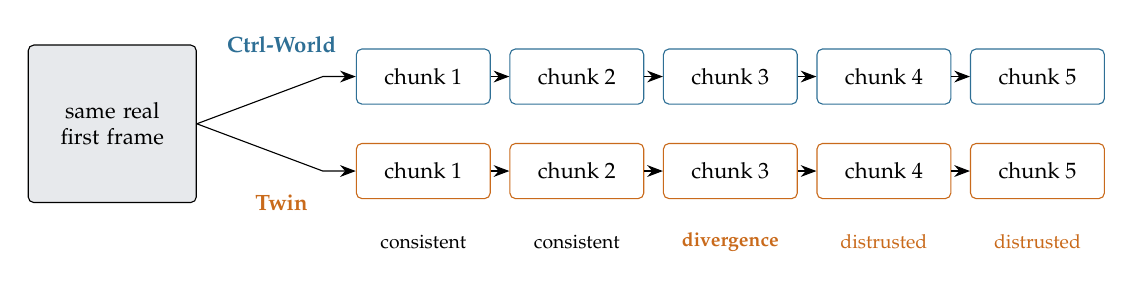
\begin{tikzpicture}[
  ch/.style={draw,rounded corners=2pt,minimum width=17mm,minimum height=7mm,font=\footnotesize},
  >={Stealth[length=2mm]}]
\node[draw,rounded corners=2pt,fill=navy!10,align=center,font=\footnotesize,minimum height=20mm,text width=19mm] (s) at (0,0) {same real\\ first frame};
\node[font=\footnotesize\bfseries,color=blue] at (2.15,1.0) {Ctrl-World};
\node[font=\footnotesize\bfseries,color=orange] at (2.15,-1.0) {Twin};
\foreach \k in {1,...,5}{
  \node[ch,draw=blue] (w\k) at (2.0+1.95*\k,0.6) {chunk \k};
  \node[ch,draw=orange] (t\k) at (2.0+1.95*\k,-0.6) {chunk \k};
}
\draw[->] (s.east) -- ++(1.6,0.6) -- (w1.west);
\draw[->] (s.east) -- ++(1.6,-0.6) -- (t1.west);
\foreach \a/\b in {1/2,2/3,3/4,4/5}{\draw[->] (w\a) -- (w\b); \draw[->] (t\a) -- (t\b);}
\node[font=\scriptsize,align=center] at (w1|-0,-1.5) {consistent};
\node[font=\scriptsize,align=center] at (w2|-0,-1.5) {consistent};
\node[font=\scriptsize,align=center,color=orange] at (w3|-0,-1.5) {\textbf{divergence}};
\node[font=\scriptsize,align=center,color=orange] at (w4|-0,-1.5) {distrusted};
\node[font=\scriptsize,align=center,color=orange] at (w5|-0,-1.5) {distrusted};
\end{tikzpicture}%

\caption{Grounded comparison. Both models run open-loop from the same real frame on the same actions; they are compared on change since frame 0. Once Ctrl-World's scene decisively leaves what the twin allows, its later rewards are computed in a scene that physics could not have produced, and are distrusted. The labels are an illustration, not a result.}
\label{method:fig:grounded}
\end{figure}

\subsubsection{Grounded disagreement and twin spread}
Let $\VW_{i,0:k}$ and $\VS_{i,0:k}(\vartheta)$ be the full videos from the start to the end of chunk $k$. Using the change since frame 0 (eq.~\ref{method:eq:change}), the grounded disagreement and the twin's own spread at chunk $k$ are
\begin{align}\label{method:eq:grounded}
d_{i,k}(\vartheta)&=\frac{1}{|\mathcal T_k|}\sum_{t\in\mathcal T_k}\big\lVert c_t(\VW_{i,0:k})-c_t(\VS_{i,0:k}(\vartheta))\big\rVert_2,\\
\kappa_{i,k}&=\max_{\vartheta,\vartheta'\in\Theta}\frac{1}{|\mathcal T_k|}\sum_{t\in\mathcal T_k}\big\lVert c_t(\VS_{i,0:k}(\vartheta))-c_t(\VS_{i,0:k}(\vartheta'))\big\rVert_2 .\notag
\end{align}
The score $S_{i,k}=\min_{\vartheta\in\Theta}d_{i,k}(\vartheta)$ asks whether \emph{any} plausible physics and start state explains Ctrl-World's change. The spread $\kappa_{i,k}$ measures how much the twin itself is unsure; it typically grows with $k$.

\subsubsection{Decision rule}
\begin{itemize}
\item The twin \textbf{abstains} at chunk $k$ if $\kappa_{i,k}>\kappa_{\max}$, or if chunk $k$ lies in a phase where the twin does not beat Ctrl-World (Step~5.2).
\item Otherwise Ctrl-World has \textbf{decisively diverged} at chunk $k$ if the normalised score exceeds the calibrated threshold, $S_{i,k}/m_k>q_\alpha$, with $m_k$ a per-chunk scale (the median calibration score, computed on the fitting half).
\item The \textbf{divergence chunk} of candidate $i$ is the first such chunk, $k^\ast_i$ ($k^\ast_i=\infty$ if none). From $k^\ast_i$ on, all its rewards are distrusted: they are computed in a scene that has left physics.
\end{itemize}

\subsubsection{Calibrating the threshold: a false-alarm guarantee that does not require a perfect twin}
For each calibration demonstration $j=1,\dots,n$ ($n=20$), the same pipeline is run with the \emph{real} video in place of Ctrl-World's: initialise the twin from the demonstration's first frame, replay its actions, and compute the trajectory score
\begin{equation}
T_j=\max_{k}\ \frac{S^{\mathrm{real}}_{j,k}}{m_k},\qquad S^{\mathrm{real}}_{j,k}=\min_{\vartheta\in\Theta_j}d^{\mathrm{real}}_{j,k}(\vartheta),
\end{equation}
over the chunks where the twin does not abstain. Set $q_\alpha$ to the $\lceil(n+1)(1-\alpha)\rceil$-th smallest $T_j$ (split conformal prediction~\cite{lei2018,angelopoulos}); with $n=20$ and $\alpha=0.1$ this is the 19th smallest.

\begin{proposition}[Controlled false alarms]\label{method:prop:conformal}
Suppose a rollout's predicted video were a real execution of its actions from its start, exchangeable with the calibration demonstrations (Assumption~\ref{method:as:exch}). Then the probability that it is flagged as diverged at \emph{any} chunk is at most $\alpha$.
\end{proposition}
\begin{proof}
The rollout is flagged at some chunk if and only if its trajectory score $T_{n+1}=\max_k S_{n+1,k}/m_k$ exceeds $q_\alpha$. Under exchangeability of $(T_1,\dots,T_{n+1})$, the rank of $T_{n+1}$ is uniform (ties broken at random), so $\Pr\big(T_{n+1}>T_{(\lceil(n+1)(1-\alpha)\rceil)}\big)\le\alpha$, the standard split-conformal bound.
\end{proof}
\begin{why}
\textbf{What this buys.} The twin does not have to be accurate for this guarantee: its imperfections show up in the calibration scores and simply raise the threshold, which costs detection power but not false alarms. What the guarantee does need is that the policy's actions look like demonstration actions to the twin (exchangeability). This is not exact, so the false-alarm rate is also measured directly on real executions of the policy (the real-robot trials of Section~\ref{method:sec:experiments}, replayed in both models).
\end{why}

\begin{proposition}[Detection under an adequate twin]\label{method:prop:detect}
Suppose (M1$'$) at the true $\vartheta^\star\in\Theta$ the twin's change differs from the real change by at most $\epsilon_S$ in the norm of eq.~\eqref{method:eq:grounded}, at chunk $k$. If Ctrl-World's change differs from the real change by more than $\epsilon_S+q_\alpha m_k$, then $d_{i,k}(\vartheta^\star)>q_\alpha m_k$.
\end{proposition}
\begin{proof}
By the triangle inequality, $d_{i,k}(\vartheta^\star)\ge\lVert c(\VW)-c(V^\ast)\rVert-\lVert c(V^\ast)-c(\VS(\vartheta^\star))\rVert>\epsilon_S+q_\alpha m_k-\epsilon_S$, averaged over $t$.
\end{proof}
Proposition~\ref{method:prop:detect} concerns the true $\vartheta^\star$; the rule flags only if \emph{every} $\vartheta$ disagrees, so large world-model errors are detected when the uncertainty set is tight, and the twin abstains (rather than flags) when it is not.

%---------------------------------------------------------------------
\subsection{Trust-weighted rewards}\label{method:sec:trust}
\subsubsection{Trust weights}
Each reward $r_{i,k}$ gets a weight $w_{i,k}\in[0,1]$, the product of a chunk-0 probe term and a grounded term:
\begin{equation}
w_{i,k}=p_{i,k}\cdot g_{i,k},\qquad
g_{i,k}=\begin{cases}w_{\min}&k\ge k^\ast_i,\\ 1&\text{otherwise},\end{cases}\qquad
p_{i,k}=1\ \ (k\ge1),
\end{equation}
\begin{equation}
p_{i,0}=\begin{cases}
1 & \text{consistent},\\
w_{\min} & \text{wrong reaction, ignores the action, or invents an effect},\\
\sigma\big(\alpha_w(\log s^W-\log s_0)\big) & \text{no verdict: world model's own consistency check},\\
1 & \text{not probed (the paper's behaviour)}.
\end{cases}
\end{equation}
$\sigma$ is the logistic function; $w_{\min}\in(0,1)$, $\alpha_w$ and $s_0$ are fixed in Step~5. Where the twin gives no verdict, the weight reflects whether Ctrl-World's response to the action exceeds its own sampling noise: if it does not, the reward difference between candidates is mostly noise. A soft grounded term (decaying with $S_{i,k}/m_k$ instead of a step) is an ablation.

\subsubsection{Neutral imputation with the trust-weighted mean}
\begin{equation}\label{method:eq:neutral}
m_k=\frac{\sum_i w_{i,k}\,r_{i,k}}{\sum_i w_{i,k}},\qquad \hat r_{i,k}=w_{i,k}\,r_{i,k}+(1-w_{i,k})\,m_k,
\end{equation}
and $\hat r$ replaces $r$ in eq.~\eqref{method:eq:adv}. Since $w_{\min}>0$, $\sum_iw_{i,k}>0$ and $m_k$ is always defined.

\begin{proposition}[Trust weighting is safe and exactly neutral]\label{method:prop:neutral}
(a) If $w\equiv1$, $\hat r=r$: the paper's method is recovered exactly. (b) $\tfrac1G\sum_i\hat r_{i,k}=m_k$. (c) A reward with $w_{i,k}=0$ contributes exactly zero to the centred returns $R_{i,k'}-\mu_{k'}$, $k'\le k$; by Lemma~\ref{method:lem:zero} it exerts no push on the policy. (d) $\hat r_{i,k}\in[\min_jr_{j,k},\max_jr_{j,k}]$: a wrong verdict can shrink a reward toward the mean, never flip or inflate it.
\end{proposition}
\begin{proof}
(a) Immediate. (b) $\sum_i\hat r_{i,k}=\sum_iw_ir_i+m_k\sum_i(1-w_i)=m_k\sum_iw_i+m_k(G-\sum_iw_i)=Gm_k$. (c) $R_{i,k'}-\mu_{k'}=\sum_{j\ge k'}\gamma^{j-k'}(\hat r_{i,j}-\tfrac1G\sum_{i'}\hat r_{i',j})$, and for $j=k$ with $w_{i,k}=0$ the term is $m_k-m_k=0$ by (b). (d) $m_k$ is a convex combination of the $r_{j,k}$, and $\hat r_{i,k}$ a convex combination of $r_{i,k}$ and $m_k$.
\end{proof}
\begin{remark}
With the plain group mean in place of $m_k$, (c) holds only approximately, because the mean of the adjusted rewards then differs from the plain mean. The trust-weighted mean makes it exact. In practice $w_{\min}>0$ keeps a small contribution, which avoids discarding information entirely when a verdict is wrong.
\end{remark}

\subsubsection{One RL iteration with the referee}
\begin{keybox}
\small
\textbf{For each group $b$ (shared real start $o_0$):}
\begin{enumerate}[label=\arabic*.]
\item Initialise the twin from $o_0$ (cached per starting scene): $\hat\X_\nu$, $\Theta=\Psi_K\times\hat\X_\nu$.
\item Run the paper's rollouts: $G$ candidates $\times$ $N$ chunks, with Ctrl-World; save Ctrl-World's state at chunk 0.
\item Run the twin on every candidate's full action sequence for every $\vartheta\in\Theta$ (MuJoCo on CPU) and render.
\item Chunk 0: for a fraction $\rho$ of candidates, generate $J$ probes; re-run Ctrl-World from the saved state with $R$ common seeds; null action once per group; compute verdicts and $p_{i,0}$.
\item All chunks: compute $S_{i,k}$, $\kappa_{i,k}$, the divergence chunk $k^\ast_i$ and $g_{i,k}$.
\item Weights $w_{i,k}=p_{i,k}g_{i,k}$; trust-weighted rewards (eq.~\ref{method:eq:neutral}); returns and advantages; FPO update.
\item Log all verdicts, scores, spreads, phases and weights (for RQ1 and RQ2).
\end{enumerate}
\end{keybox}

%---------------------------------------------------------------------
\subsection{Diagnostics used only for analysis}\label{method:sec:diag}
\begin{itemize}
\item \textbf{Arm-following check.} The commanded end-effector path is known. In free space, the arm visible in Ctrl-World's frames is compared with the robot twin rendered at the commanded pose, $e^{\mathrm{arm}}=1-\IoU(\text{arm mask in }\VW,\text{rendered arm})$. A large value means Ctrl-World did not follow the actions, which would confound every other comparison.
\item \textbf{False imagined successes.} The twin has an explicit state. A rollout that the success classifier judges successful on Ctrl-World's video, while the lid angle stays above the closing threshold for every $\vartheta\in\Theta$ in the twin, is a \emph{physically inconsistent success}. Its share over updates is the most direct measure of exploitation (RQ2). This uses the twin's state for analysis only, never in the training signal.
\item \textbf{Re-synchronised residual (optional).} Re-initialising the twin from Ctrl-World's frame at chunk $k$ and checking whether any plausible physics explains its transition to chunk $k+1$ localises \emph{when} an error occurs. Because it reads states from generated frames, it is used only to interpret RQ2, not for training.
\end{itemize}

%=====================================================================
\renewcommand{\thesubsection}{\thesection.\arabic{subsection}}
\renewcommand{\thesubsubsection}{\thesubsection.\arabic{subsubsection}}
\section{Assumptions and how each is tested}\label{method:sec:assumptions}
%=====================================================================
The guarantees above are relative to these assumptions. Each is tested on data that exist before any RL run, or on the real robot at the end.
\begin{assumption}[Model adequacy]\label{method:as:adequacy}
The twin's structure reproduces the sign of real effects, and (M1$'$) its change is close to the real change in the phases where it is used. \emph{Test:} demonstration replays per phase (Step~5.2); real action pairs (Section~\ref{method:sec:exp-real}).
\end{assumption}
\begin{assumption}[Coverage]\label{method:as:coverage}
The true physics and start state lie in $\Theta$. \emph{Test:} share of held-out replays whose real change lies within the twin's envelope; leave-one-view-out IoU of the initialiser.
\end{assumption}
\begin{assumption}[Controller fidelity]\label{method:as:ctrl}
The twin executes actions like the real robot. \emph{Test:} commanded versus measured poses in the demonstrations (delay, tracking error).
\end{assumption}
\begin{assumption}[Exact restore]\label{method:as:restore}
Ctrl-World's state can be saved and restored exactly. \emph{Test:} same state, same seed, same action gives identical output.
\end{assumption}
\begin{assumption}[Representation validity]\label{method:as:rep}
$\Dt$ responds more to physical change than to appearance change. \emph{Test:} Step~5.4.
\end{assumption}
\begin{assumption}[Support]\label{method:as:support}
Probes and the null action stay where Ctrl-World was trained. \emph{Test:} $\tilde a\in\mathcal A_{\mathrm{demo}}$ by construction; near-still segments exist in the demonstrations for $a_\varnothing$.
\end{assumption}
\begin{assumption}[Exchangeability]\label{method:as:exch}
For the false-alarm guarantee, policy rollouts resemble demonstrations as seen by the twin. \emph{Test:} false-alarm rate measured on real policy executions replayed in both models.
\end{assumption}

\begin{center}\small
\begin{tabularx}{\linewidth}{@{}>{\raggedright\arraybackslash}p{4.2cm}>{\raggedright\arraybackslash}X@{}}
\toprule
\textbf{Proven (well-posedness)} & only rankings matter (L\ref{method:lem:shift}); zero advantage gives zero push (L\ref{method:lem:zero}); the fit exists (P\ref{method:prop:fit}); $\Dt$ is a bounded pseudometric that cancels constant offsets (P\ref{method:prop:dt}); everything is bounded (L\ref{method:lem:bound}); identification of the action effect (P\ref{method:prop:ident}); small probes exist (P\ref{method:prop:probe}); the null verdict needs no physics (P\ref{method:prop:null}); sign errors controlled (P\ref{method:prop:signW}); labels are a partition (P\ref{method:prop:partition}); trust weighting is safe and exactly neutral (P\ref{method:prop:neutral}).\\
\midrule
\textbf{Guaranteed under assumptions} & decisive chunk-0 verdicts are correct under M1--M2 (P\ref{method:prop:sound}); false divergence flags at most $\alpha$ under M7 (P\ref{method:prop:conformal}); large errors detected under M1$'$ (P\ref{method:prop:detect}).\\
\midrule
\textbf{Empirical (the thesis's results)} & whether M1--M7 hold and where; how often each verdict occurs; whether failures grow and precede the decline; whether trust weighting improves real success.\\
\bottomrule
\end{tabularx}
\end{center}

%=====================================================================
\section{Experiments}\label{method:sec:experiments}
%=====================================================================

\subsection{E0 · Referee validation, before RL (G1)}
\begin{itemize}
\item \textbf{Initialiser} on real first frames of all four tasks: leave-one-view-out IoU; lid-angle error (degrees) and position error (cm) on about 10 labelled frames per task; share of frames flagged as ambiguous.
\item \textbf{Replay of the 40 laptop demonstrations} in the twin and in Ctrl-World from their real first frames with their real actions: error of each against the real video, per phase; envelope coverage (M2).
\item \textbf{Representation and appearance checks} (Step~5.4); exact-restore check (M4).
\end{itemize}

\subsection{E1 · Audit of the original method (RQ1, G2)}
On rollouts of the original method (arm A below, with all checks computed but $w\equiv1$):
\begin{itemize}
\item verdict rates per type (consistent, wrong reaction, ignores the action, invents an effect, no verdict), per phase and per starting scene;
\item candidate-pair ranking agreement between Ctrl-World and twin on decisive pairs;
\item null-action hallucination rate per group;
\item grounded divergence: distribution of the divergence chunk $k^\ast$; abstention rate per chunk;
\item arm-following error $e^{\mathrm{arm}}$ in free space.
\end{itemize}

\subsection{E2 · Training dynamics (RQ2, G2)}
Over the updates of arm A: failure and divergence rates versus update; model-space success from the paper's classifier; share of physically inconsistent imagined successes (Step~9). Tests: trend over updates (Mann--Kendall), and whether the increase in failures leads the drop in model-space success (lagged cross-correlation across updates and seeds). The optional re-synchronised residual localises when errors occur.

\subsection{E3 · Training arms (RQ3, G3)}
All arms use the same rollout and update budget.
\begin{center}\small
\begin{tabularx}{\linewidth}{@{}lX@{}}
\toprule
\textbf{Arm} & \textbf{What it tests}\\
\midrule
A: original FPO & Baseline at our budget; also the data source for E1--E2. The authors' released RL checkpoint is a second reference.\\
T: full trust weighting & The proposed method: chunk-0 verdicts and grounded divergence.\\
T0: chunk-0 only & Contribution of the per-action verdicts ($g\equiv1$).\\
TG: grounded only & Contribution of the later-chunk check ($p\equiv1$).\\
S: shuffled weights & The weights of T, randomly permuted within each batch: separates \emph{which} rewards are down-weighted from \emph{how many}.\\
\bottomrule
\end{tabularx}
\end{center}
All arms are run at a reduced profile with two seeds; A and the best trust-weighted arm are then run at the full profile. Metrics in imagination: model-space success over updates, presence and timing of the late decline, share of physically inconsistent successes.

\subsection{E4 · Real-world demonstrations}\label{method:sec:exp-real}
\textbf{Main demonstration (G3).} Laptop closing on the UR5: the paper's RL policy versus the best trust-weighted policy, about 60 trials each, with the same set of laptop placements for both policies, in randomised order, using the paper's protocol (success rate and completion time). If time allows, the SFT policy is added as a lower reference. With 60 trials per policy, a difference from 68\% to 90\% is detected with about 85\% power (two-sided, $\alpha=0.05$); smaller gains are reported as estimates with 95\% confidence intervals ($\pm$12 percentage points at 68\%).

\textbf{Which model gets reality right? (G2).} About 20 pairs (action $a$, probe $\tilde a$) are executed from identical starts on the UR5, with the actions taken from the policy at chunk 0 on the real first frame. For each pair, the real effect $\tau^{\mathrm{real}}=Q^{\mathrm{real}}(v,a)-Q^{\mathrm{real}}(v,\tilde a)$ is computed with the same score as the models, and its sign is compared with $\tau^W$ and with the twin's decisive verdict. Five repeats of the same action measure the real noise floor and the repeatability of the placement (checked with the initialiser).

\textbf{Post-hoc use of the trials (no extra robot time).} Each recorded real trial is replayed open-loop in Ctrl-World and in the twin from its first frame with its executed actions. This measures, on real policy actions at scale, (i) how often Ctrl-World's predicted change departs from reality, (ii) the false-alarm rate of the divergence test (Assumption~\ref{method:as:exch}), and (iii) whether flagged rollouts are those where Ctrl-World is actually wrong.

\textbf{Execution.} Robot sessions are run by lab members with a written protocol, scripts, a placement sheet and automatic video and log recording, prepared and tested before robot access begins. Total robot time is about 5--6 hours.

%=====================================================================
\section{Goals, deliverables and real-world demonstrations}\label{method:sec:deliverables}
%=====================================================================
\begin{center}\small
\begin{tabularx}{\linewidth}{@{}>{\raggedright\arraybackslash}p{2.7cm}>{\raggedright\arraybackslash}X>{\raggedright\arraybackslash}X@{}}
\toprule
\textbf{Goal} & \textbf{Deliverable} & \textbf{Real-world demonstration and metric}\\
\midrule
\textbf{G1 · Physics referee} & MuJoCo twin of the UR5 laptop cell; initialiser from the first frame (SAM\,3 masks, fit of base pose and lid angle); V-JEPA comparison; integrated in the paper's RL code; released as open code. & Initialiser on real first frames of all four tasks: lid-angle error ($^\circ$), position error (cm), held-out-view IoU. The 40 laptop demos replayed in twin and Ctrl-World: error against the real video, per contact phase.\\
\midrule
\textbf{G2 · Audit} (RQ1, RQ2) & Verdict log for every reward over the RL runs; error rates by type, phase and training step; share of physically inconsistent imagined successes over training. & About 20 (action, perturbed action) pairs on the UR5 from identical starts: measured effect versus both models' predictions. Replays of all real trials in both models.\\
\midrule
\textbf{G3 · Trust-weighted training} (RQ3) & Trust-weighted FPO on the action head with ablations; trained laptop-closing checkpoint. & Paper's policy versus ours, about 60 trials each, identical placements: success rate with 95\% confidence interval.\\
\bottomrule
\end{tabularx}
\end{center}

%=====================================================================
\section{Expected results}\label{method:sec:expected}
%=====================================================================
\begin{center}\small
\begin{tabularx}{\linewidth}{@{}>{\raggedright\arraybackslash}p{2.6cm}>{\raggedright\arraybackslash}X>{\raggedright\arraybackslash}p{4.4cm}@{}}
\toprule
\textbf{Question} & \textbf{Expected result} & \textbf{Measured by}\\
\midrule
Referee (G1) & The twin initialises itself on all four tasks without manual work, and is closer to reality than Ctrl-World during and after contact. & Held-out-view IoU, labelled errors; demo replays (E0).\\
RQ1 · Detect & Ctrl-World contradicts physics in a clear share of decisive cases (at least 10\%), mostly around contact; ``ignores the action'' and ``invents an effect'' are the most frequent failure types. & Verdicts on training rollouts (E1).\\
RQ2 · Explain & Failure and divergence rates grow during training and precede the drop in imagined success; physically inconsistent successes increase. & Verdicts across updates (E2).\\
RQ3 · Improve & No late decline in imagination; real success at least the paper's 68\% on laptop closing, with a clear gain as target; the shuffled control does not improve. & Training curves (E3); UR5 trials (E4).\\
\bottomrule
\end{tabularx}
\end{center}

\paragraph{Interpretation of possible outcomes.}
\begin{itemize}
\item \emph{Few errors found (RQ1 negative).} The world model is reliable on this task; the decline has another cause, e.g.\ degrading plans. The referee and the audit are still delivered, and RQ3 is expected to be neutral.
\item \emph{Errors found but not growing.} The world model is wrong but not exploited; trust weighting acts as noise reduction, with a smaller expected gain.
\item \emph{Errors grow and precede the decline.} Evidence of exploitation; RQ3 tests whether removing that feedback fixes it.
\item \emph{RQ3 negative despite RQ1--RQ2 positive.} Down-weighting alone may remove too much signal; the coverage of verdicts and the share of distrusted rewards are reported to diagnose this.
\end{itemize}

%=====================================================================
\section{Risks and fallbacks}\label{method:sec:risks}
%=====================================================================
\begin{center}\small
\begin{tabularx}{\linewidth}{@{}>{\raggedright\arraybackslash}p{5.2cm}>{\raggedright\arraybackslash}X@{}}
\toprule
\textbf{Risk} & \textbf{Mitigation}\\
\midrule
V-JEPA distances dominated by render-versus-generated appearance & Textured rendering from the real first frame; change features; appearance floor; representation check (Step~5.4); fallback to silhouette comparison with SAM\,3 masks.\\
The twin is not more accurate than Ctrl-World in any phase & The demo-replay comparison is itself a result (G1); the method then reduces to the world model's own consistency check, and RQ1--RQ2 use real trials replayed in both models.\\
The twin abstains too often (low coverage) & Report coverage per phase and chunk; tighten $p(\psi)$ with more demos; use chunk-0 verdicts only.\\
Initialiser fails on some frames or tasks & Quality gate excludes them; report the failure rate; manual initialisation for the few laptop starting scenes if needed.\\
Missing calibration or robot states in the data & Estimate camera extrinsics from the rendered robot; check the data in the first two weeks.\\
Ctrl-World state cannot be restored exactly & Re-run from the saved observation and history with fixed seeds; measure residual nondeterminism and include it in $\sigma^W$.\\
Ctrl-World rarely disagrees with physics & Report it (outcome 1); focus RQ2 on the other possible causes of the decline.\\
Cluster queue time & Reduced profiles; early submission; audit on logged rollouts; the twin runs on CPUs.\\
Robot time only at the end, executed remotely & Protocol and scripts prepared and dry-run in advance; post-hoc replays need no extra robot time; ask whether a short session can be brought forward.\\
\bottomrule
\end{tabularx}
\end{center}

%=====================================================================
\section{Compute and robot-time budget}\label{method:sec:budget}
%=====================================================================
\paragraph{Extra Ctrl-World calls.} With probe fraction $\rho$, $J$ probes and $R$ seeds per probed candidate at chunk 0, the extra calls per iteration are $B\,G\,\rho\,\big((J+1)R-1\big)$, against $B\,G\,N$ for the paper ($B$ groups). With $J=R=2$: $+25\%$ for $\rho=0.25$, $+50\%$ for $\rho=0.5$. The grounded comparison needs no extra Ctrl-World calls.
\paragraph{Twin and features.} MuJoCo rollouts and rendering for $|\Theta|$ elements per candidate (subsampled to about 16) run on CPUs in parallel with Ctrl-World. V-JEPA features at low resolution are small next to Cosmos and Ctrl-World.
\paragraph{Runs.} Five arms at a reduced profile with two seeds, plus two full runs: well within the monthly cluster allocation; queue time is the limiting factor.
\paragraph{Robot.} 120 evaluation trials, about 20 action pairs and the repeats: about 5--6 hours, executed by lab members.

%=====================================================================
\section{Work plan}\label{method:sec:plan}
%=====================================================================
\begin{center}\small
\begin{tabularx}{\linewidth}{@{}>{\raggedright\arraybackslash}p{3.1cm}>{\raggedright\arraybackslash}X>{\raggedright\arraybackslash}p{4.6cm}@{}}
\toprule
\textbf{Period} & \textbf{Work} & \textbf{Checkpoint}\\
\midrule
15 Oct -- 4 Nov & Reproduce a reduced laptop run on the cluster with full logging; check the data (videos, robot states, actions, calibration); boundary statement. & Pipeline runs; data sufficient.\\
5 Nov -- 2 Dec & General twin, initialiser, rendering, V-JEPA comparison; Ctrl-World save/restore. & G1 initialiser validated on four tasks.\\
3 Dec -- 16 Dec & Calibration on demonstrations (Step~5): $p(\psi)$, phase map, thresholds, representation check. & Twin beats Ctrl-World in at least one phase; checks pass, otherwise fallbacks.\\
17 Dec -- 13 Jan & Arm A with full audit (E1--E2); arms T, T0, TG, S at reduced profile. & RQ1, RQ2 results.\\
14 Jan -- 24 Jan & Full runs of A and the best arm; freeze policies; robot protocol and scripts dry-run. & Policies frozen.\\
25 Jan -- 8 Feb & Robot sessions (E4), executed by lab members; replays of the trials. & Real-world results.\\
whole period, focus 1 -- 19 Feb & Writing. & Hand-in 19 Feb 2027.\\
\bottomrule
\end{tabularx}
\end{center}

%=====================================================================
\section{Open decisions with the supervisor}\label{method:sec:decisions}
%=====================================================================
\begin{enumerate}
\item \textbf{Data.} Confirm that the released demonstrations contain multi-view videos, robot states, executed actions and camera calibration (or that extrinsics can be estimated as in Step~1).
\item \textbf{Probe budget.} Probe fraction $\rho$ ($0.25$ or $0.5$), trading compute for verdict coverage.
\item \textbf{Robot sessions.} Who in the lab runs them, and whether a short session for the action pairs can take place before 25 January.
\item \textbf{Scope of the four-task validation.} Initialiser only (proposed), or also demonstration replays on a second task.
\item \textbf{Boundary statement} with the colleague's thesis, agreed in writing at the start.
\end{enumerate}

% Back to the book's numbering for the chapters that follow.
\renewcommand{\thesection}{\thechapter.\arabic{section}}

% Chapter 04. Source: docs/book/import/twin_walkthrough.tex, ported in D.2 without rewriting.
% Skeleton from WP D.1: the section headings below are the source's; D.2 replaces them with its
% body (the source's two appendices become the last sections).
\chapter{The scene digital twin, from data to referee}\label{ch:twin}

\section{What the twin is, and what it is for}

\section{The life cycle: four moments}

\section{The data the twin needs}

\section{MuJoCo in two pages, and how the twin is stored}

\section{Frames and conventions}

\section{The components, one by one}

\section{End to end: one episode, from the dataset to the weight}

\section{How it plugs into the training code}

\section{Status and what comes next}

\section{Shapes cheat sheet}

\section{Glossary}

% Chapter 05. Step 8 itself (trust weights, neutral imputation, one RL iteration with the referee) is
% in chapter 03 and is not repeated here (O17, option (a), decided 27 Nov 2026). This chapter holds
% decision D1: docs/thesis/notes/d1_scale_policy.md converted to LaTeX in D.2 without rewriting.
% Its references to the proposal ("Eq. (20)", "P14 (b)", ...) are links to chapter 03, which prints
% the proposal's numbers. The Markdown note stays in docs/thesis/notes/; change both together.
\chapter{Trust weighting}\label{ch:trust}

The trust weights and the neutral imputation with the trust-weighted mean are Step~8 of the
proposal, \cref{method:sec:trust}; they are not repeated here. This chapter holds decision D1 of the
implementation plan: which standard deviation scales the trust-weighted advantages. The proposal's
eq.~\eqref{method:eq:adv} uses the std of the trust-weighted returns (option A); option B, the std of
the raw returns, is an extra ablation (data-free roadmap, §0.1).

\section{D1: which std scales the trust-weighted advantages}\label{trust:sec:d1}

Companion to \code{src/rlinf\_modified/algorithms/trust.py} and \code{tests/test\_trust\_weighting.py}
(WP 1.2, 25 Nov 2026). Equation and proposition numbers refer to the proposal (27 Oct 2026).

\subsection{Setup}

Fix one group of $G$ candidates. Weights $w_{i,k}\in(0,1]$. Eq.~\eqref{method:eq:neutral}:
\[
m_k=\frac{\sum_i w_{i,k}r_{i,k}}{\sum_i w_{i,k}},\qquad \hat r_{i,k}=w_{i,k}r_{i,k}+(1-w_{i,k})\,m_k .
\]
Suffix returns $\hat R_{i,k}=\sum_{j\ge k}\gamma^{j-k}\hat r_{i,j}$ and raw returns $R_{i,k}$ (same
with $r$). Centred returns $C_{i,k}=\hat R_{i,k}-\frac1G\sum_{i'}\hat R_{i',k}$. ``Std'' is the
unbiased std (as in the code), so $\sum_i C_{i,k}^2=(G-1)\,\mathrm{Std}_i(\hat R_{i,k})^2$.

\begin{itemize}
\item \textbf{A} (eq.~\eqref{method:eq:adv}, default): $\hat A_{i,k}=C_{i,k}/(\hat s_k+\epsilon)$ with
  $\hat s_k=\mathrm{Std}_i\hat R_{i,k}$.
\item \textbf{B} (ablation): $\hat A_{i,k}=C_{i,k}/(s_k+\epsilon)$ with $s_k=\mathrm{Std}_i R_{i,k}$.
\end{itemize}

One identity is used throughout. By P\ref{method:prop:neutral}~(b), the group mean of
$\hat r_{\cdot,k}$ is $m_k$, so
\begin{equation*}
\hat r_{i,k}-m_k=w_{i,k}\,(r_{i,k}-m_k).\tag{$*$}\label{trust:eq:star}
\end{equation*}

\subsection{Test 5: Lemma 1 holds after imputation, for A and B}

Add $c_j$ to every reward of the group at chunk $j$. Then $m_j\to m_j+c_j$, so
$\hat r_{i,j}\to w(r+c_j)+(1-w)(m_j+c_j)=\hat r_{i,j}+c_j$. Every imputed reward moves by the same
$c_j$, as do the raw rewards. Every $\hat R_{i,k}$ and every $R_{i,k}$ then moves by the same
$\sum_{j\ge k}\gamma^{j-k}c_j$. So $C$, $\hat s_k$ and $s_k$ are unchanged, and so are the advantages
under A and under B.

The shift may differ between groups, because everything is computed per group.
\textbf{Condition:} the done boundaries must be shared within a group (fixed horizon). A member
whose episode ended before chunk $j$ would not receive $c_j$. The test uses dones only at the end;
whether production dones are always shared within a group is \chk.

\subsection{Test 6, option A: the total is fixed at \texorpdfstring{$G-1$}{G-1}}

$\sum_i \hat A_{i,k}^2=(G-1)\,\hat s_k^2/(\hat s_k+\epsilon)^2=(G-1)\,(1-O(\epsilon/\hat s_k))$,
whatever the weights.

Distrust therefore cannot change the total; it only redistributes it. By \eqref{trust:eq:star},
distrusted members' centred rewards shrink toward 0, so the trusted members carry a larger share.
If $G_T$ members are trusted and typical, each has $\hat A^2\approx (G-1)/G_T$ instead of
$(G-1)/G$: a factor $\sqrt{G/G_T}$, which is 2 for 12 of 16 distrusted.

\subsection{Test 6, option B: a fixed scale and a bound at the last chunk}

\textbf{(i) The scale does not depend on the weights.} $s_k$ is computed from the raw returns, so
$\hat A_{i,k}(s_k+\epsilon)=C_{i,k}$ exactly. The weights move the centre and the imputed values,
never the scale.

\textbf{(ii) At the last chunk, distrust never increases the total.} At $k=N-1$,
$C_{i,k}=\hat r_{i,k}-m_k=w_{i,k}(r_{i,k}-m_k)$ by \eqref{trust:eq:star}. Write $\bar r_k$ for the
plain mean. Then
\[
\sum_i C_{i,k}^2=\sum_i w_i^2(r_i-m)^2\ \le\ \sum_i w_i(r_i-m)^2\ \le\ \sum_i w_i(r_i-\bar r)^2\ \le\
\sum_i (r_i-\bar r)^2=(G-1)s_k^2 .
\]
The first and last steps use $w\le1$. The middle step holds because $m$ minimises
$\sum_i w_i(r_i-c)^2$ over $c$. Hence $\sum_i\hat A_{i,k}^2\le (G-1)s_k^2/(s_k+\epsilon)^2$, the
value at full trust. The same holds at every chunk when $\gamma=0$.

\textbf{(iii) At earlier chunks the bound fails.} $C_{i,k}=\sum_{j\ge k}\gamma^{j-k}w_{i,j}(r_{i,j}-m_j)$
(from \eqref{trust:eq:star}, using $\sum_i(\hat r_{i,j}-m_j)=0$). Each chunk's vector shrinks, but
cancellation across chunks in the raw returns can be undone.

Example: $G=2$, $r_0=(1,-1)$, $r_1=(-1,1)$, $\gamma=0.95$, $w_1=0.05$ for both members.
\begin{itemize}
\item Raw: $C_0=\pm0.05$.
\item Imputed: $C_0=\pm0.9525$.
\item The total grows about 360 times ($|\hat A|$ goes from 0.71 to 13.5).
\end{itemize}

\subsection{What does not hold: per-member monotonicity}

``The trusted members' advantages do not grow when others are distrusted'' is false under both
policies. Example: $G=16$, rewards eight 0 and eight 10, seven of the zeros distrusted with
$w=0.05$. The trusted zero-member's $|\hat A|$ is:

\begin{center}
\begin{tabular}{@{}lccc@{}}
\toprule
 & Full trust & B & A\\
\midrule
trusted zero-member $\lvert\hat A\rvert$ & 0.97 & 1.66 & 3.47\\
\bottomrule
\end{tabular}
\end{center}

Distrust moves $m_k$ toward the trusted majority, so away from a trusted minority member. B keeps
the scale, but the centre still moves. The test
\code{test\_d1\_counterexamples\_per\_member\_growth\_and\_earlier\_chunks} pins this example and the
one in (iii).

\subsection{Side result: exact neutrality of the advantages holds only under A}

With $w_{i,k}=0$, $r_{i,k}$ drops out of $\hat r$ entirely (P\ref{method:prop:neutral}~(c)), so out
of $C$ for both policies. Under A it then drops out of the advantages too. Under B it still enters
through $s_k$, so changing it rescales the whole group. With $w_{\min}>0$ neither policy is exact.

\subsection{Summary}

\begin{center}
\small
\begin{tabularx}{\linewidth}{@{}lYY@{}}
\toprule
 & A (eq.~\eqref{method:eq:adv}, default) & B (ablation)\\
\midrule
Scale & std of imputed returns, depends on $w$ & std of raw returns, independent of $w$\\
$\sum_i \hat A^2$ per chunk & $= G-1$ always & $\le$ full-trust value at the last chunk; can grow earlier\\
Effect of heavy distrust & same total update, concentrated on fewer members & smaller total update at the last chunk\\
$w=0$ reward & no effect on the advantages & no effect on $C$; still sets the scale\\
Per member & can grow (e.g.\ 3.6$\times$ above) & can grow (e.g.\ 1.7$\times$ above)\\
\bottomrule
\end{tabularx}
\end{center}

Interpretation for the optimisation notes \chk:
\begin{itemize}
\item Under A, the FPO surrogate keeps its overall magnitude whatever the trust. With little trust,
  the update is driven by a few members, so its variance rises.
\item Under B, heavy distrust shrinks the last-chunk advantages, which is more conservative, at the
  cost of a reward scale that still contains the distrusted rewards.
\end{itemize}

% Chapter 06. Short: the decisions marked Approved in docs/thesis/open_items_and_deviations.md (§2,
% and the resolved items of §1.4), with a pointer to that file for the rest (D.2). When a decision is
% approved, add it here (definition of done, item 3 in CLAUDE.md).
\chapter{Decisions}\label{ch:decisions}

Every departure from the plan, with what the plan says, what was done instead, why, and whether it
was approved, is tracked in \code{docs/thesis/open\_items\_and\_deviations.md}. ``The plan'' means,
in order of precedence, the proposal (\cref{ch:proposal}), the data-free roadmap, the implementation
plan and the detailed guide. This chapter lists only the decisions marked \emph{Approved} there,
as of 27 November 2026.

\section{Approved decisions}

{\small
\begin{longtable}{@{}p{2.3cm}>{\raggedright\arraybackslash}p{10.6cm}p{2.6cm}@{}}
\toprule
\textbf{Where} & \textbf{Decision} & \textbf{Approved}\\
\midrule
\endhead
T1 & Robot model: the original UR5, generated from the DH constants in
\code{eef\_pose\_adapter.py}, not the UR5e of MuJoCo Menagerie. Those constants produced
Ctrl-World's conditioning states; the proposal allows adapting to the older UR5. &
roadmap §0.1\\
T2 & Resampling 15 to 30\,Hz: rotation by quaternion slerp, through the repo function
\code{resample\_eef\_state\_sequence\_by\_fps} called as is, not linear in the axis-angle channels. &
repo behaviour\\
T2 & The action conversion runs in float32, as production does, which gives bit-exact parity. &
repo behaviour\\
T2 & Camera roles: main = \code{d405\_0\_rgb}, wrist = \code{d435\_rgb}, side = \code{d405\_1\_rgb}
(\code{camera\_layout.py}), not as in the implementation plan and the guide. & 17 Nov\\
WP 1.2 & Roadmap acceptance 6 for D1-B is replaced by its provable version: B's scale does not
depend on the weights, and at the last chunk $\sum_i\hat A_{\mathrm B}^2$ never exceeds its
full-trust value; the counterexample to the original claim is pinned in a test
(\cref{trust:sec:d1}). & 25 Nov\\
WP 1.4 & The no-verdict probe weight has a floor:
$p=\max\bigl(w_{\min},\sigma(\alpha_w(\log s_W-\log s_0))\bigr)$. It equals
eq.~(19) wherever $\sigma(\cdot)\ge w_{\min}$. & 26 Nov\\
WP 1.4 & One $s_W$ per candidate (a scalar argument); the rule for $J$ probes is left to WP 2.2. &
26 Nov\\
WP 1.5 & $w=p\cdot g$ is not clipped, as in eq.~(18): $w\in[w_{\min}^2,1]$. &
26 Nov\\
WP 1.5 & The soft grounded term (Step 8.1 ablation) is
$g_k=w_{\min}+(1-w_{\min})\,\sigma\bigl((q_\alpha-R_k)/\mathrm{scale}\bigr)$, with $R_k$ the running
maximum of $S_j/m_j$ over the non-abstaining chunks $j\le k$. & 26 Nov\\
WP D.1 & Zoomable diagrams in the code docs (buttons, wheel, drag, full screen). & 26 Nov\\
WP D.2 & Step 8 appears once, in \cref{ch:proposal}; \cref{ch:trust} links to it and holds only the
D1 note (O17, option (a)). & 27 Nov\\
WP D.2 & \Cref{ch:proposal} holds the proposal's Sections 1--14 with ``The proposal in brief'',
numbered as in the proposal; its Notation is \cref{method:app:notation}, its references close the
book. & 27 Nov\\
WP D.2 & \code{twin\_code\_map.tex} is not in the book: the code docs (\code{docs/code/}) are its
maintained version. & 27 Nov\\
WP D.2 & \code{scripts/make\_book\_figures.py} writes the four images of \cref{ch:rl-to-fpo} into
\code{docs/book/figures/} by default. & 27 Nov\\
WP D.2 & The book is compiled locally with TinyTeX (TeX Live in user space); CI uses its own TeX
Live image. & 27 Nov\\
\bottomrule
\end{longtable}}

\section{Everything else}

The open items (what needs a decision, a lab answer or a later check), the choices marked
\emph{Review} (made during a work package and not yet confirmed) and the errors found in the plan
documents are only in \code{docs/thesis/open\_items\_and\_deviations.md}. The running log of what is
done, with test results, is \code{docs/thesis/progress.md}.


\appendix
% Appendix A. Source: the appendix "Notation" of import/thesis_proposal_final.tex, ported in D.2
% without rewriting; its \section heading is a \chapter here (the book's appendix).
\chapter{Notation}\label{method:app:notation}
%=====================================================================
\small
\begin{longtable}{@{}p{3.0cm}p{12.6cm}@{}}
\toprule
\textbf{Symbol} & \textbf{Meaning}\\
\midrule
\multicolumn{2}{@{}l}{\emph{Paper's loop}}\\
$k$, $N=5$ & chunk index and number of chunks per rollout.\\
$i$, $G=16$; $B$ & candidate in a group and group size; number of groups per iteration.\\
$o_k$, $g$ & observation (three camera images) at chunk $k$; language instruction.\\
$\Pi_\theta$, $\theta_a$ & world-action model (Cosmos); trained action-head parameters.\\
$z$, $D$ & latent sample and decoder, $D(z)=(\VC,a)$.\\
$\VC_{i,k}$, $a_{i,k}$ & imagined plan video; action chunk ($H_a=32$ steps at 15\,Hz, $d_a=10$).\\
$W$, $h$, $\xi$, $T_a$ & Ctrl-World, its conditioning state, sampling noise, action conversion.\\
$\VW_{i,k}$, $\mathrm{Ext}$ & predicted video; takes its last frame as next observation.\\
$r_{i,k}$, $D_{\mathrm{pix}}$, $I^\star_g$ & reward, pixel MSE, goal image.\\
$\gamma$, $R_{i,k}$, $\mu_k$, $s_k$, $\hat A_{i,k}$ & discount, return, group mean and standard deviation, advantage.\\
$\rho$, $\epsilon_{\mathrm{clip}}$ & FPO ratio and clipping threshold (in Section~\ref{method:sec:budget}, $\rho$ is the probe fraction).\\
\midrule
\multicolumn{2}{@{}l}{\emph{Twin and initialiser}}\\
$q,\dot q$; $x\in\X$ & robot joints and velocities; object configuration, for the laptop $(p_x,p_y,\varphi,\vartheta)$.\\
$\psi$, $p(\psi)$, $\Psi_K$ & uncertain physical parameters, their belief, $K$ samples.\\
$F_\psi$, $T_S$, $\mathrm{Rend}_v$ & twin dynamics over one chunk, action conversion, renderer of camera $v$.\\
$K_v$, $T_v$ & camera intrinsics and extrinsics.\\
$\VS$ & twin video.\\
$M^{\mathrm{obs}}_v$, $M_v(x;q)$ & SAM\,3 masks; rendered masks.\\
$\mathcal L$, $\hat x$, $\hat\X_\nu$, $\nu$, $\mathcal L_{\max}$ & fitting loss, its minimiser, near-optimal set, tolerance, quality gate.\\
$\Theta=\Psi_K\times\hat\X_\nu$, $\vartheta$ & uncertainty set of the twin and one element (physics and start state).\\
\midrule
\multicolumn{2}{@{}l}{\emph{Comparison, verdicts and trust}}\\
$\phi_t$, $\phi_{\mathrm{ref}}$, $c_t$ & V-JEPA feature of the window ending at $t$; of a still clip of the first frame; change since frame 0.\\
$\Dt$, $Q^M$ & change-based distance; score of an action under a plan in model $M\in\{W,S\}$.\\
$\tilde a$, $\varepsilon$, $B$, $c$; $a_\varnothing$ & probe, size, displacement basis, direction; null action.\\
$\tau^W$, $\tau^S(\vartheta)$, $\tau^{\mathrm{real}}$ & effect of replacing $a$ by $\tilde a$ in Ctrl-World, twin, reality.\\
$\eta_0$, $\eta$ & ``no effect'' and ``effect'' thresholds of the twin.\\
$\sigma^W$, $s^W$, $s_0$ & pooled Ctrl-World noise scale, effect size, significance threshold.\\
$d_{i,k}$, $S_{i,k}$, $\kappa_{i,k}$, $\kappa_{\max}$ & grounded disagreement, its minimum over $\Theta$, twin spread, abstention threshold.\\
$m_k$ (Step 7), $q_\alpha$, $k^\ast_i$ & per-chunk scale, conformal threshold, divergence chunk.\\
$p_{i,k}$, $g_{i,k}$, $w_{i,k}$, $w_{\min}$, $\alpha_w$ & probe term, grounded term, trust weight, floor, slope.\\
$m_k$ (Step 8), $\hat r_{i,k}$ & trust-weighted group mean of rewards; trust-weighted reward.\\
\bottomrule
\end{longtable}
\normalsize


\backmatter
% The references of import/thesis_proposal_final.tex, unchanged (D.2). Cited in chapter 03;
% \input at the end of main.tex. \bibname is set to the proposal's heading in preamble.tex.
\cleardoublepage\phantomsection\addcontentsline{toc}{chapter}{\bibname}
\begin{thebibliography}{99}\small
\bibitem{a2a} Y.~Qiao, Z.~Wei, et al. Achieve What You Imagined: Learning to Align Actions with Visual Plans. arXiv:2609.33832, 2026.
\bibitem{ctrlworld} Y.~Guo, L.~X.~Shi, J.~Chen, C.~Finn. Ctrl-World: A Controllable Generative World Model for Robot Manipulation. ICLR 2026, arXiv:2510.10125.
\bibitem{cosmos3} NVIDIA. Cosmos 3: Omnimodal World Models for Physical AI. arXiv:2606.02800, 2026.
\bibitem{fpo} D.~McAllister, S.~Ge, et al. Flow Matching Policy Gradients. 2025.
\bibitem{vjepa2} M.~Assran et al. V-JEPA 2: Self-Supervised Video Models Enable Understanding, Prediction and Planning. arXiv:2506.09985, 2025.
\bibitem{sam3} Meta AI. SAM 3: Segment Anything with Concepts. 2025. \url{https://github.com/facebookresearch/sam3}.
\bibitem{sam3d} Meta AI. SAM 3D Objects. 2025. \url{https://github.com/facebookresearch/sam-3d-objects}.
\bibitem{mujoco} E.~Todorov, T.~Erez, Y.~Tassa. MuJoCo: A Physics Engine for Model-Based Control. IROS 2012.
\bibitem{menagerie} K.~Zakka, Y.~Tassa, and MuJoCo Menagerie contributors. MuJoCo Menagerie. \url{https://github.com/google-deepmind/mujoco_menagerie}.
\bibitem{mopo} T.~Yu et al. MOPO: Model-based Offline Policy Optimization. NeurIPS 2020.
\bibitem{exploitable} Imperfect World Models are Exploitable. arXiv:2605.15960, 2026.
\bibitem{lei2018} J.~Lei, M.~G'Sell, A.~Rinaldo, R.~J.~Tibshirani, L.~Wasserman. Distribution-Free Predictive Inference for Regression. JASA 113(523), 2018.
\bibitem{angelopoulos} A.~N.~Angelopoulos, S.~Bates. A Gentle Introduction to Conformal Prediction and Distribution-Free Uncertainty Quantification. arXiv:2107.07511, 2021.
\bibitem{realissim} Real-is-Sim: Bridging the Sim-to-Real Gap with a Dynamic Digital Twin for Real-World Robot Policy Evaluation. arXiv:2504.03597.
\bibitem{vptwin} VPTwin: Real-Sim-Real Video Prediction for Robotic Manipulation Planning. arXiv:2609.33104, 2026.
\bibitem{wmpo} WMPO: World Model-based Policy Optimization for Vision-Language-Action Models. ICLR 2026, arXiv:2511.09515.
\end{thebibliography}


\end{document}
